\section{Generating Code for Patterns}

\subsection{Introduction}

To be able to generate code for patterns, three kinds of functions are required.

\begin{enumerate}
\item
\texttt{IsA} function that accepts a term and returns a boolean if it matches the desired pattern. This is done by ensuring that each term instance is of an expected class (e.g. \texttt{Integer}) and additionally verifying side conditions (e.g. \texttt{natural} term must of class \texttt{Integer} and its value must be greater or equal to zero). All \texttt{IsA} functions have the following signature:

\begin{minted}[tabsize=2,obeytabs,escapeinside=||,mathescape=true,fontsize=\normalsize]{python}
isA(term: Term) -> boolean
\end{minted}

\item
The matching function that accepts a \texttt{Match} instance, a \texttt{Term} instance, and two extra arguments \texttt{head} and \texttt{tail} which indicate a range of subterms in the term that haven't been matched yet. Successful matching increments value of \texttt{head} by one. In principle it should be possible to perform pattern matching bi-directionally but PyPltRedex doesn't implement this. All matching functions have the following signature:

\begin{minted}[tabsize=2,obeytabs,escapeinside=||,mathescape=true,fontsize=\normalsize]{python}
matchfunc(match: Match, term: Term, head: int, tail: int) -> [(Match, int, int)]
\end{minted}

\item
The top-level matching function that accepts a \texttt{Term} instance, initializes \texttt{Match} with pattern-variables found in the pattern and calls matching procedure. \texttt{Match} instances are then filtered and returned. All top-level matching functions have the following signature:
\begin{minted}[tabsize=2,obeytabs,escapeinside=||,mathescape=true,fontsize=\normalsize]{python}
toplevel_matchfunc(term: Term) -> [Match]
\end{minted}
\end{enumerate}


\subsection{Is-A Functions}

\texttt{IsA} functions are generated for all built-in patterns excluding \texttt{InHole} patterns.  Originally, most of these procedures were generated by PyPltRedex dynamically but then I realized these could just the part of the runtime library introduced in Chapter \ref{chapter04}. This allowed for greater code generator simplification.

\begin{figure}[H]
\begin{minted}[tabsize=2,obeytabs,escapeinside=||,mathescape=true,linenos,fontsize=\normalsize]{python}
def term_is_number(term):
    return isinstance(term, Float) or isinstance(term, Integer)

def term_is_integer(term):
    return isinstance(term, Integer)

def term_is_float(term):
    return isinstance(term, Float)

def term_is_natural_number(term):
    return isinstance(term, Integer) and term.value() >= 0

def term_is_hole(term):
    return isinstance(term, Hole)

def term_is_string(term):
    return isinstance(term, String)

def term_is_boolean(term):
    return isinstance(term, Boolean)

def term_is_variable_not_otherwise_mentioned(term, variableset):
    return isinstance(term, Variable) and term.value() not in variableset
\end{minted}
\caption{\texttt{IsA} functions for all built-in datatypes.}
\label{codegen-builtin-isa}
\end{figure}

The figure above shows the \texttt{IsA} procedures for \texttt{number}, \texttt{real}, \texttt{natural}, \texttt{string}, \texttt{boolean} and \texttt{variable-not-otherwise-mentioned} patterns. All of these use Python's built-in \texttt{isinstance} function to check if given term is of proper subclass of \texttt{Term} described in Section \ref{section:runtime-terms}.

Most of these functions can be called directly. The only function that looks different is \texttt{term\_is\_variable\_not\_otherwise\_mentioned} and that is because a set of variables used by related \texttt{define-language} form is required and is not known until compile time. This is solved by creating a wrapper function.

This completes the description of \texttt{IsA} functions. \texttt{IsA} functions are also generated for each non-terminal definition in \texttt{define-language} form and their generation will be explained later.

\subsection{Matching Functions: Literals}
Matching $p=$\LiteralPattern \space is very similar to \texttt{IsA} functions described above - they first check if passed \texttt{term} is of expected class and then compare value of the term to the value $v$, passed in the place of \texttt{literal} parameter. These functions are also a part of the runtime library and can be seen in Figure \ref{codegen-pat-literal}.

\begin{figure}[H]
\begin{minted}[tabsize=2,obeytabs,escapeinside=||,mathescape=true,linenos,fontsize=\normalsize]{python}
def consume_literal_integer(term, match, head, tail, literal):
    if isinstance(term, Integer) and term.value() == literal:
        return [ (match, head+1, tail) ]
    return []

def consume_literal_float(term, match, head, tail, literal):
    if isinstance(term, Float) and abs(literal - term.value()) < 0.001:
        return [ (match, head+1, tail) ]
    return []

def consume_literal_string(term, match, head, tail, literal):
    if isinstance(term, String) and term.value() == literal:
        return [ (match, head+1, tail) ]
    return []

def consume_literal_boolean(term, match, head, tail, literal):
    if isinstance(term, Boolean) and term.value() == literal:
        return [ (match, head+1, tail) ]
    return []

def consume_variable(term, match, head, tail, literal):
    if isinstance(term, Variable) and term.value() == literal:
        return [ (match, head+1, tail) ]
    return []
\end{minted}
\caption{Functions that match literals in a pattern.}
\label{codegen-pat-literal}
\end{figure}

Since functions do not conform to the previously described interface, a wrapper function is generated, calling one of the functions based on $kind$, as seen in Figure \ref{codegen-lit-code}.

\begin{figure}[H]
\begin{minted}[tabsize=2,obeytabs,escapeinside=||,mathescape=true,linenos,fontsize=\normalsize]{python}

	
	
def |$f_p$|(match, term, head, tail):
	return |$consume_p$|(term, p.|$v$|)


\end{minted}
\caption{Generated function for a \LiteralPatternNoArg pattern}
\label{codegen-lit-code}
\end{figure}

\subsection{Matching Functions: Built-In Patterns and Non-terminals}
Given \BuiltInPattern \space or \NonTerminal \space and equipped with \texttt{IsA} functions defined above (also assuming \texttt{isa} functions for non-terminal definitions have been generated), upon successful application of appropriate \texttt{isa} procedure, \texttt{head} must be incremented by one and term must be assigned to pattern-variable $s$. The choice of \texttt{isa} procedure depends on $t$.

Generated code does the following:

\begin{enumerate}
\item Call appropriate \texttt{IsA} procedure.
\item If result is True, add term to the \texttt{match} under appropriate pattern-variable, increment \texttt{head} by one and return a list containing \texttt{(match, head, tail)} tuple.
\item Otherwise, return an empty list.
\end{enumerate}
\begin{figure}[H]
\begin{minted}[tabsize=2,obeytabs,escapeinside=||,mathescape=true,linenos,fontsize=\normalsize]{python}

	
	
def |$f_p$|(match, term, head, tail):
	tmp0 = |$isa_p$|(term)
	if tmp0 == True:
		tmp1 = match.addtobinding(|$s$|, term)
		head = head + 1
		return [(match, head, tail)]
return []


\end{minted}
\caption{Matching built-in patterns and non-terminal symbols.}
\label{codegen-builtin-nt-1}
\end{figure}

\subsection{Matching Functions: Repeat}
\label{section:pattern-repeat}
Recall that patterns under ellipsis match lists of terms and can only be contained in pattern sequences and thus \texttt{term} argument is always to be expected to be \PatternSequence. Given $p=$ \PatternRepeat \space pattern, non-deterministic matching repetition of terms is handled in the following way. Let $pv_1^{(p)}, ..., pv_n^{(p)}$ be a set pattern-variables assigned in $p_r$. These are read from \texttt{PatternVariables} annotation.  Let $f_p$ be matching function for $p$ with usual parameters. Generate  matching function for $p_r$, $f_{p_r}$.

\begin{enumerate}
\item
For each symbol in $pv_i^{p}$, call \texttt{match.increasedepth} method. Functionality of \texttt{increasedepth} was described in Section \ref{section:Match}.
\item
Pack \texttt{match}, \texttt{head}, \texttt{tail} back into a tuple, and initialize lists \texttt{matches} and \texttt{queue} containing said tuple. \texttt{matches} will eventually contain all the matches produced by $f_p$. \texttt{queue} contains matches that are yet to be processed. Since $p_r$ can be non-deterministic, $f_{p_r}$ needs to be applied for every match in \texttt{queue}.
\item The following is repeated until \texttt{queue} is empty.
	\begin{enumerate}
	\item
	Remove \texttt{(m, h, t)} from the queue. If \texttt{h == t} then all elements of the sequence have been matched and there's nothing left to do.
	\item
	Retrieve an element at index \texttt{head} of the term sequence and call $f_{p_r}$ with resulting \texttt{Match} instance after calling \texttt{m.deepcopy}.
	\item Append resulting list of matches to \texttt{matches} and \texttt{queue}.
	\end{enumerate}

\item
For each obtained \texttt{(m, h, t)} in \texttt{matches} call \texttt{m.decreasedepth} method with $pv_i^{p}$. This completes matching the list of terms. \texttt{matches} is returned.
\end{enumerate}

\begin{figure}
\begin{minted}[tabsize=2,obeytabs,escapeinside=||,mathescape=true,fontsize=\normalsize]{python}

	
	
	
def |$f_p$|(term, match, head, tail):
	:
	match.increasedepth(|$pv_i^{p}$|)
	
	matchtuple = (match, head, tail)
	matches, queue = [matchtuple], [matchtuple]
	while len(queue) != 0:
		m, h, t = queue.pop(0)
		if h == t: continue
		m = m.copy()
		newmatches =|$f_{p_r}$|(term.get(h), m, h, t)
	matches, queue = matches + newmatches, queue + newmatches
	:
	for (m, h, t) in matches:
		m.decreasedepth(|$pv_i^{p}$|)
	
	return matches

\end{minted}
\caption{Matching repetition of terms \RepeatNoArg \space in \texttt{Sequence}.}
\label{codegen-pattern-ellipsis-1}
\end{figure}


\subsection{Matching Functions: PatternSequence}
Given $p = $\PatternSequence, generate matching functions $f_{p_1}, ..., f_{p_n}$ for patterns $p_1, ..., p_n$. Code generation for pattern sequences is more involved and a requires a bit of setup.

\begin{enumerate}
\item
First, ensure that the \texttt{term} is a \texttt{Sequence}.  Then, the term has to be "entered" to be ready for matching; that is, to be able to use $f_{p_i}$ to match subterms new values for \texttt{head} and \texttt{tail} are required. Initialize \texttt{nhead = 0}` and set \texttt{ntail} to be length of the term sequence - these will be used to track which elements of the \texttt{Sequence} haven't been matched yet.
\item Before matching elements of the term, ensure that the number of these elements is greater or equal to the number of elements in the \texttt{PatternSequence}, excluding patterns under ellipses and constraint checking nodes.
\item \texttt{Sequence} is now ready to be matched - create an empty list of matches and initialize it with \texttt{(match, ntail, nhead)} tuple.
\item
Depending on the kind of pattern $p_i$, different matching strategies are required and are to be explained later. For now, assume all the patterns $p_i$ have been matched.
\item
After matching all patterns $p_i$, \texttt{TermSequence} has to be "exited"; that is, original \texttt{head} and \texttt{tail} have to be restored. Let \texttt{matches\_m} be a list of matches after matching the last pattern $p_n$. For each resulting match tuple (m, h, t) in \texttt{matches\_m}, need to ensure that \texttt{h = t}, that is all terms in \texttt{TermSequence} have been matched. If that is the case, tuple \texttt{(m, head+1, tail)} is appended to the list of resulting matches, indicating that \texttt{TermSequence} itself has been matched.
\end{enumerate}
Figure \ref{codegen-pattern-seq-1} demonstrates this.

\begin{figure}[htb]
\centering
\begin{minted}[tabsize=2,obeytabs,escapeinside=||,mathescape=true,fontsize=\normalsize]{python}

	
	
	
def |$f_p$|(term, match, head, tail):
	if not isinstance(term, Sequence): return []
	subtail, subhead = 0, term.length()
	if subtail - subhead < $n$ : return []
	|$matches_0$|= [(match, subtail, subhead)]
	
		
			#snip
		
			#snip
		
			#snip
		
	outmatches = []
	for m, h, t in matches_m:
		if m == t:
			outmatches.append((m, head+1, tail))
	return outmatches

\end{minted}
\caption{Setting up \texttt{Sequence} for pattern matching.}
\label{codegen-pattern-seq-1}
\end{figure}

Now, different code is emitted for different kinds of $p_i$.

\begin{itemize}
\item $p_i=$ \PatternRepeat. Matching function $f_{p_i}$ is called with \texttt{term} (i.e. \texttt{Sequence}) for each \texttt{(m,h,t)} in $matches_{i-1}$. Results of matching is accumulated into list $matches_{i}$. Additionally, ensure that the remaining number of terms in the \texttt{Sequence} is greater than the remaining number of non-optional patterns to be matched; that is $n-i$. Matches that pass this test are accumulated into list $matches_{i+1}$ Finally, ensure that $matches_{i+1}$ is non-empty, otherwise return an empty list. Figure \ref{codegen-pattern-seq-2} demonstrates this.

\begin{figure}[htb]
\centering
\begin{minted}[tabsize=2,obeytabs,escapeinside=||,mathescape=true,fontsize=\normalsize]{python}

	
|$matches_i$| = []
for m, h, t in |$matches_{i-1}$|:
	|$matches_i$| = |$matches_i$| + |$f_{p_i}$|(term, m, h, t)
	
	
		
|$matches_{i+1}$| = []
for m, h, t in |$matches_{i}$|:
	if tail - head >= $r$:
		|$matches_{i+1}$|.append((m, h, t))
if len(|$matches_{i+1}$|) == 0: return []
	
\end{minted}
\caption{Matching \RepeatNoArg \space in \texttt{Sequence}.}
\label{codegen-pattern-seq-2}
\end{figure}

\item $p_i=$ \PatternCheckConstraint. For each \texttt(m, h, t) in $matches_{i-1}$, ensure that \texttt{m.comparekeys} succeeds for $sym_1$ and $sym_2$ and accumulate succeding matches into $matches_{i}$. Additionally, check if list $matches_{i}$ is non-empty otherwise return. Figure \ref{codegen-pattern-seq-3} demonstrates this.


\begin{figure}[htb]
\centering
\begin{minted}[tabsize=2,obeytabs,escapeinside=||,mathescape=true,fontsize=\normalsize]{python}

	
|$matches_i$| = []
for m, h, t in |$matches_{i-1}$|:
	if m.comparekeys(|$sym_1$|, |$sym_2$|):
		|$matches_i$|.append((m, h, t))
if len(|$matches_i$|) == 0: return []
\end{minted}
\caption{Handling \ConstraintCheckNoArg \space while matching \texttt{Sequence}.}
\label{codegen-pattern-seq-3}
\end{figure}

\item Any other pattern kind $p_i$, given list of matches $matches_{i-1}$, call $f_{p_i}$ for each \texttt{(m, h, t)} in $match_{i-1}$ with term at position \texttt{h} and accumulate resulting matches into new list $match_{i}$. If $match_{i}$ is empty, matching \texttt{TermSequence} has failed and empty list is returned. Figure \ref{codegen-pattern-seq-3} demonstrates this.

\begin{figure}[htb]
\begin{minted}[tabsize=2,obeytabs,escapeinside=||,mathescape=true,fontsize=\normalsize]{python}


|$matches_i$| = []
for m, h, t in |$matches_{i-1}$|:
	|$matches_i$| = |$matches_i$| + |$f_{p_i}$|(term.get(h), match, h, t)
if len(|$matches_i$|) == 0: return []

\end{minted}
\caption{Handling any another pattern in \PatternSequenceNoArg \space while matching \texttt{Sequence}.}
\label{codegen-pattern-seq-3}
\end{figure}
\end{itemize}

\subsection{Match Functions: InHole}
Given pattern \PatternInHole, let $f_p^{impl}$ name of the function for \texttt{in-hole} pattern. Recall that \texttt{in-hole} pattern is annotated with pattern-variables during "Pattern Variable Extraction" pass described in Section \ref{section:pv-extraction}. Let $pv_i^{(p_1)}$ and $pv_i^{(p_2)}$ be annotations for $p_1$ and $p_2$. Finally, generate functions for $p_1$ and $p_2$ and let them be $f_{p_1}$ and $f_{p_2}$ respectively.

Notice that this function contains an extra parameter \texttt{path}, which is used to keep track of path to possible \texttt{hole}. To conform to the established interface, a wrapper function will be generated later.

Since $p_1$ and $p_2$ are self-contained patterns with possible non-deterministic behavior, \texttt{match} cannot be passed to $f_{p_1}$ and $f_{p_2}$ as is. Instead, create special \texttt{Match} instances to be passed to $f_{p_1}$ and $f_{p_2}$ that are initialized with $pv_i^{(p_1)}$ or $pv_i^{(p_2)}$ accordingly.

First, call $f_{p_2}$ with appropriate match, if resulting list of matches is non-empty, do the following: (1) append current term to the path; (2) call path copying function thus replacing the term with \texttt{hole} and (3) call $f_{p1}$ with appropriate match. If resulting set of matches is not empty, increment \texttt{head} (without overwriting it!) by one signaling successful matching of \texttt{in-hole} pattern, combine resulting matches of $f_{p_1}$ and $f_{p_2}$ with initial \texttt{match} as explained in Section \ref{section:Match}, and append to \texttt{matches}.

If the given \texttt{term} is \texttt{Sequence}, continue matching \texttt{in-hole} pattern. Each element of the sequence is added to the path, $f_p^{impl}$ is called with said element, resulting matches are added to \texttt{matches} and topmost term in the \texttt{path} is popped. Resulting \texttt{matches} are returned. This logic is shown in Figure \ref{pat-inhole-1}.

\begin{figure}[H]
\begin{minted}[tabsize=2,obeytabs,escapeinside=||,mathescape=true,fontsize=\normalsize]{python}

	
	
	
	
def |$f_p$|(term, match, head, tail, path):
	matches = []
	p2match = Match([|$pv_1^{(p_2)}, ..., pv_m^{(p_2)}$|])
	p2ms = |$f_{p_2}$|(term, p2match, 0, 1)
	if len(p2ms) != 0:
		p1match = Match(|$pv_1^{(p_1)}, ..., pv_n^{(p_1)}$|)
		npath = path + [term]
		nterm = copy_path_and_replace_last(tmp0, hole)
		p1ms = |$f_{p_1}$|(nterm, p1match, 0, 1)
		if len(p1ms) != 0:
			nhead = head + 1
			ms = match_cartesian_product_add_binding_to(
				p1ms, p2ms, match, nhead, tail)
			matches = matches + ms
	if isinstance(term, Sequence):
		path.append(term)
		for i in range(term.length()):
			childterm = term.get(i)
			results= |$f_p^{impl}$|(childterm, match,
								    head, tail, path)
			matches = matches + results
		path.pop()
	 return matches
# continued below
\end{minted}
\caption{Code for \PatternInHoleNoArg \space pattern.}
\label{pat-inhole-1}
\end{figure}

Finally, to get rid of the \texttt{path} parameter from the signature of $f_p^{impl}$, a wrapper function $f_p$ is generated. Additionally, it also handles constraint checks $c_i$ if applicable. Since constraint checks are optional, there are two cases to consider.

\begin{enumerate}
\item No constraint checks - simply return \texttt{matches}
\item Constraint checks are present - for each \PatternCheckConstraint \space generate a call to \texttt{comparekeys} method with $sym_1$ and $sym_2$. This is done for each \texttt{Match} instance returned by calling $f_p^{impl}$.
\end{enumerate}

\begin{figure}
\begin{minted}[tabsize=2,obeytabs,escapeinside=||,mathescape=true,fontsize=\normalsize]{python}
# continued from above.
	
def |$f_p$|(term, match, head, tail):
	matches = |$f_p^{impl}$|(match, head, tail, [])
	
	nmatches = []
	for m, h, t in matches:
		
	if not m.comparekeys(|$s_1$|, |$s_2$|):
		continue
	nmatches.append((m, h, t))
		
	return nmatches
	
	return matches
	
	

\end{minted}
\caption{Generation of wrapper function for \PatternInHoleNoArg \space pattern, continued from Figure \ref{pat-inhole-1}.}
\label{pat-inhole-2}
\end{figure}

\subsection{Top-Level Matching Functions}
Given some pattern $p$, generating a top-level function for a pattern involves the following steps:

\begin{itemize}
\item Retrieve a set of pattern-variables $pv_1^{p}, ..., pv_n^{p}$ assigned in the pattern from annotation \texttt{PatternVariables}.
\item Retrieve a set of pattern-variables $pvr_1^{p}, ..., pvr_m^{p}$ that are to be removed after matching from annotation \texttt{PatConstraintCheckRemoveVars} (see Section \ref{section:constraint-check}).
\item Let $f_p$ be the top-level function for pattern $p$.
\item Generate matching function $fm_p$ for pattern $p$.
\end{itemize}

Now, we get to the code-generation. Initialize \texttt{Match} object with pattern-variables $pv_i^{p}$ and call $f_p$ with said \texttt{Match} instance, \texttt{head} and \texttt{tail} set to zero and one, respectively. After a list of matches is returned, need to strip out resulting \texttt{Match} from \texttt{(Match, int, int)}  tuples as well as remove symbols $pvr_i^{p}$ from \texttt{Match} instances. Resulting \texttt{Match} instances are appended to an array. The array is then returned.


\begin{figure}
\begin{minted}[tabsize=2,obeytabs,escapeinside=||,mathescape=true,fontsize=\normalsize]{python}

	
	
	
	
def |$f_p$|(term):
	match = Match(|$pv_1^{p}, ..., pv_n^{p}$|)
	matches = |$fm_p$|(term, match, 0, 1)
	ret = []
	for m, h, t in matches:
	
		m.removekey(|$pvr_i^{p}$|}
		ret.append(m)
	
	return ret

\end{minted}
\caption{Generation of top-level matching function for pattern $p$.}
\label{pat-toplevel}
\end{figure}

\subsection{Repeat: Example}
Given pattern `((number ...) ...)` and term `((1 2 3)())`, the matching algorithm should return `Match` instance with `number = ((1 2 3)())`, i.e. the pattern matches the term exactly. The diagram below shows how using `increasedepth` and `decreasedepth` methods provided by `Match` facilitate the matching. 


\begin{figure}[h]
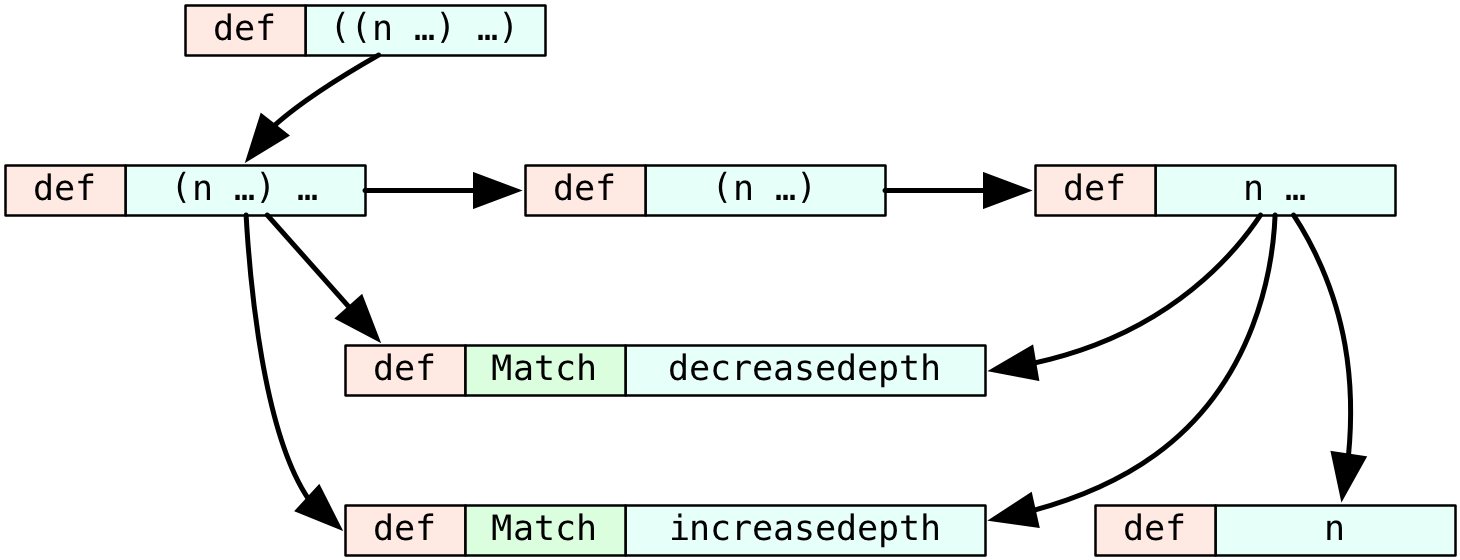
\includegraphics[scale=0.25]{ellipsis-example-callgraph.png}
\caption{Callgraph for function matching pattern \texttt{((n ...) ...)}}
\label{ellipsis-example-callgraph}
\end{figure}

Callgraph for function matching pattern \texttt{((n ...) ...)} can be seen in Figure \ref{ellipsis-example-callgraph}. Code generation algorithm generates five matching functions for this pattern:

\begin{enumerate}
\item function for pattern \texttt{((n ...) ...)}
\item function for pattern \texttt{(n ...) ...}
\item function for pattern \texttt{(n ...) }
\item function for pattern \texttt{n ... }
\item function for pattern \texttt{n}
\end{enumerate}


Figure \ref{ellipsis-example-fig-a} show state of \texttt{Match} object before beggining to match a term (red nodes) against a pattern (blue nodes). Outlined pattern nodes represent current sub-pattern being matched; and since matching hasn't begun yet the entire pattern is outlined.Same applies to the term. Initially, \texttt{Binding} instance assigned to pattern variable \texttt{n} in \texttt{Match} instance has an empty stack.

Figure \ref{ellipsis-example-fig-b} shows state of \texttt{Match} object after entering generated function for \textit{outer} ellipsis and calling \texttt{increasedepth("n")} method. This pushes empty \texttt{TermSequence} onto the stack.


Figure \ref{ellipsis-example-fig-c} shows state of \texttt{Match} object after entering generated function for \textit{inner} ellipsis and calling \texttt{increasedepth("n")} method. This pushes empty \texttt{TermSequence} onto the stack. The term now contains two \texttt{TermSequence} instances.

Figure \ref{ellipsis-example-fig-d} shows matching of term \texttt{Integer(1)}. Need to call \texttt{addtobinding} method with \texttt{"n"} and \texttt{Integer(1)} as arguments. Since topmost term on the stack is \texttt{TermSequence}, \texttt{Integer(1)} is appended to it.

Figures \ref{ellipsis-example-fig-e} and \ref{ellipsis-example-fig-f} call \texttt{addtobinding} with \texttt{Float(2.01)} and \texttt{Integer(3)}. Both terms are appended to the topmost \texttt{TermSequence} on the stack.

All terms in \texttt{TermSequence} have been consumed. Figure \ref{ellipsis-example-fig-g} shows state of the match object after calling \texttt{decreasedepth("n")}. Since the stack contains to \texttt{TermSequence} instances, topmost one is removed from stack and appended to the first \texttt{TermSequence}. Function for \textit{inner} ellipsis is exited.

Now, remaining empty term sequence has to be matched, as seen in Figure \ref{ellipsis-example-fig-h}.

Figure \ref{ellipsis-example-fig-i} shows state of \texttt{Match} object after entering generated function for \textit{inner} ellipsis. Empty \texttt{TermSequence} instance is pushed onto the stack.

However, since term sequence is empty, function for \texttt{Number} pattern cannot be called. Figure \ref{ellipsis-example-fig-j} shows state of the \texttt{Match} object after calling \texttt{decreasedepth("n")}. Since stack contains two \texttt{TermSequence} instances, topmost one is popped from the stack and appended to previous \texttt{TermSequence}. Function for \textit{inner} ellipsis is exited.

Finally, there's no more terms to match in outermost sequence and \texttt{decreasedepth("n")} has to be called, as shown in Figure \ref{ellipsis-example-fig-k}. Since the stack only contains a single term, \texttt{decreasedepth} has no effect.

Assignment \texttt{n = ((1 2 3)())} is matched, as expected.

One may notice that this example doesn't cover non-determinism when matching patterns under ellipsis. When matching term \texttt{(1 2 3)} against pattern \texttt{n ...} (as shown in Figures \ref{ellipsis-example-fig-d}, \ref{ellipsis-example-fig-e}, \ref{ellipsis-example-fig-f}), the matches shown in Figure \ref{ellipsis-example-matches-1} are returned. Recall that when calling a function that matches \texttt{TermSequence}, \texttt{head} and \texttt{tail} are set to zero and the length of \texttt{TermSequence}, in this case three. Function for \texttt{n ...} is then called, \texttt{increasedepth} method is called on \texttt{match} instance and it is placed into the queue. Match is then popped from the queue, add function for pattern \texttt{n} is called with complete copy of the match. Such repeated copying and calling \texttt{decreasedepth} for each resulting match produces matches shown in Figure \ref{ellipsis-example-matches-1}. Now, when exiting function for pattern \texttt{(n ...)}, only accept matches where \texttt{head=tail}, and there's only such match.

When control flow returns to function for pattern \texttt{(n ...) ...)}, the only returned match is added to the queue. Queue at this point contains a single match. This match is dequeued, and function for pattern \texttt{(n ...) is called} with term \texttt{()}. \texttt{head} and \text{tail} are set to zero and function for pattern \texttt{n ...} is called. \texttt{increasedepth} is called. Since term \texttt{()} contains no numbers, the only possible match returned by this function is shown in Figure \ref{ellipsis-example-matches-2}.

Finally, \textit{outer} ellipsis produces matches shown in Figure \ref{ellipsis-example-matches-3} When returning from function for pattern \texttt{((n ...) ...)}, two of the matches are discarded because \texttt{head != tail}.


\begin{figure}[H]
\caption{Lifetime of match object}
%\begin{adjustwidth}{-1cm}{1cm}
\fbox{
	\begin{subfigure}{0.5\linewidth}
		\raisebox{5mm}{
			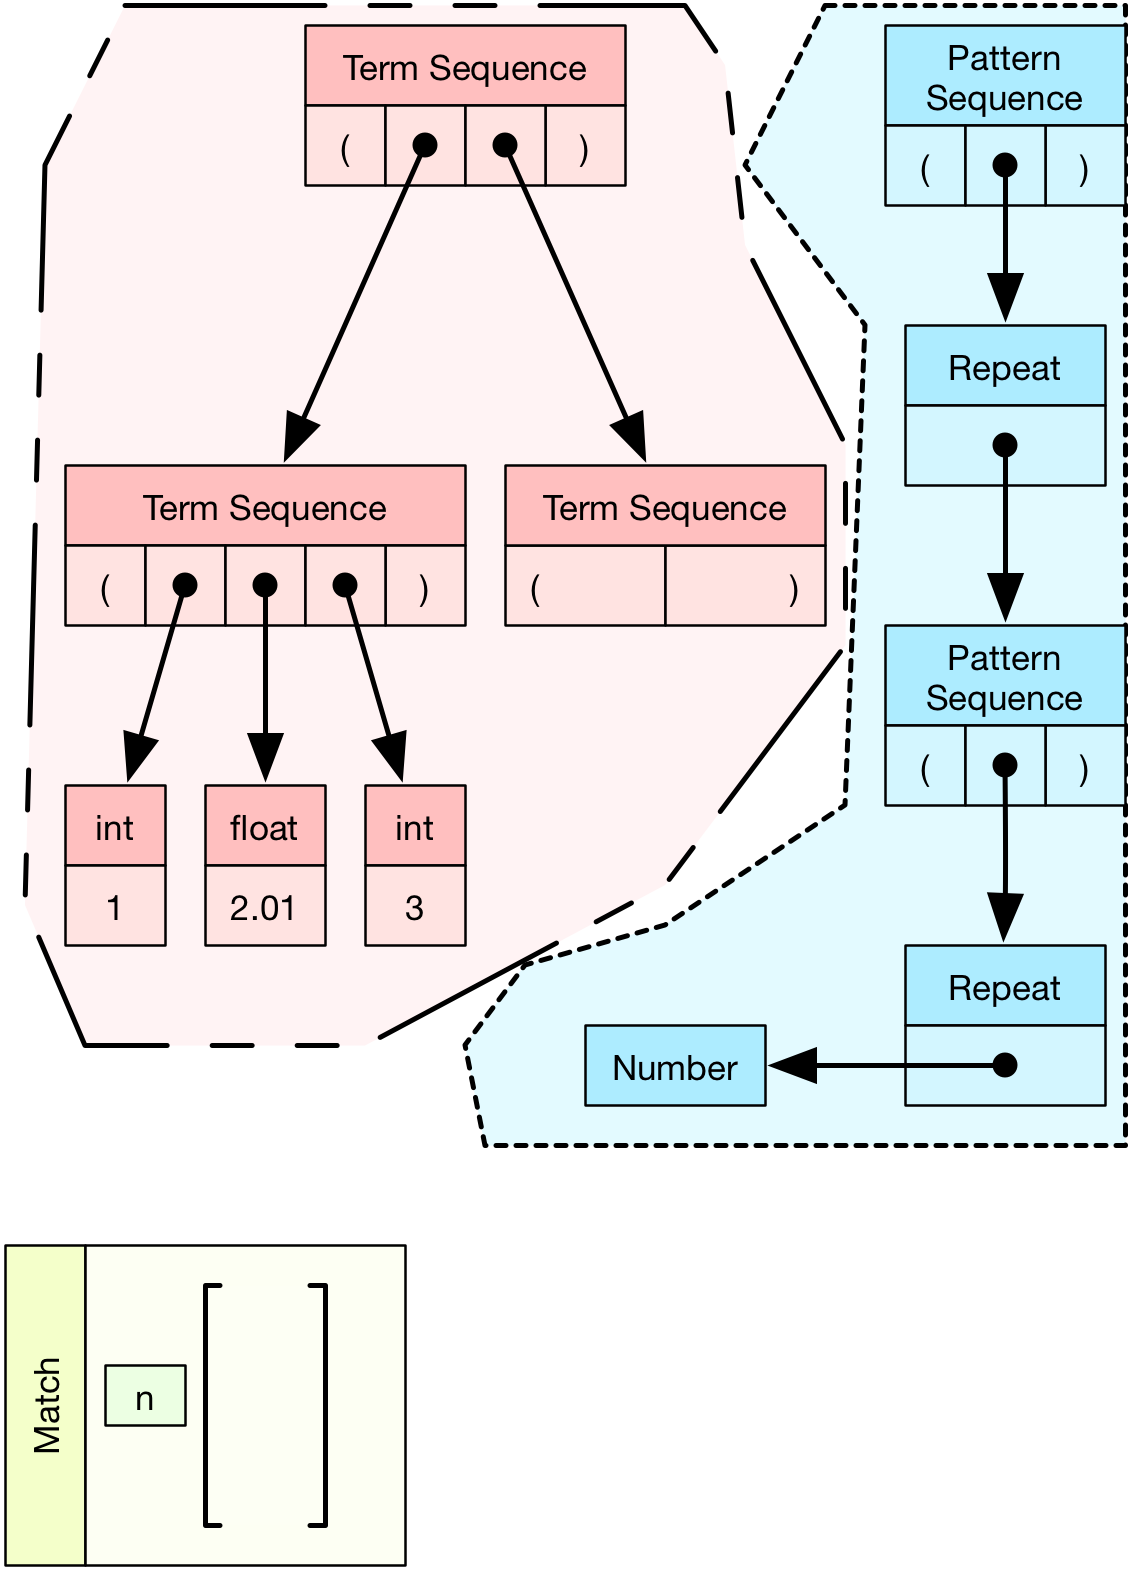
\includegraphics[scale=0.152]{ellipsis-example-fig-a.png}
		}
		\caption{Before matching the pattern.}
		\label{ellipsis-example-fig-a}
	\end{subfigure}
	\begin{subfigure}{0.5\linewidth}
		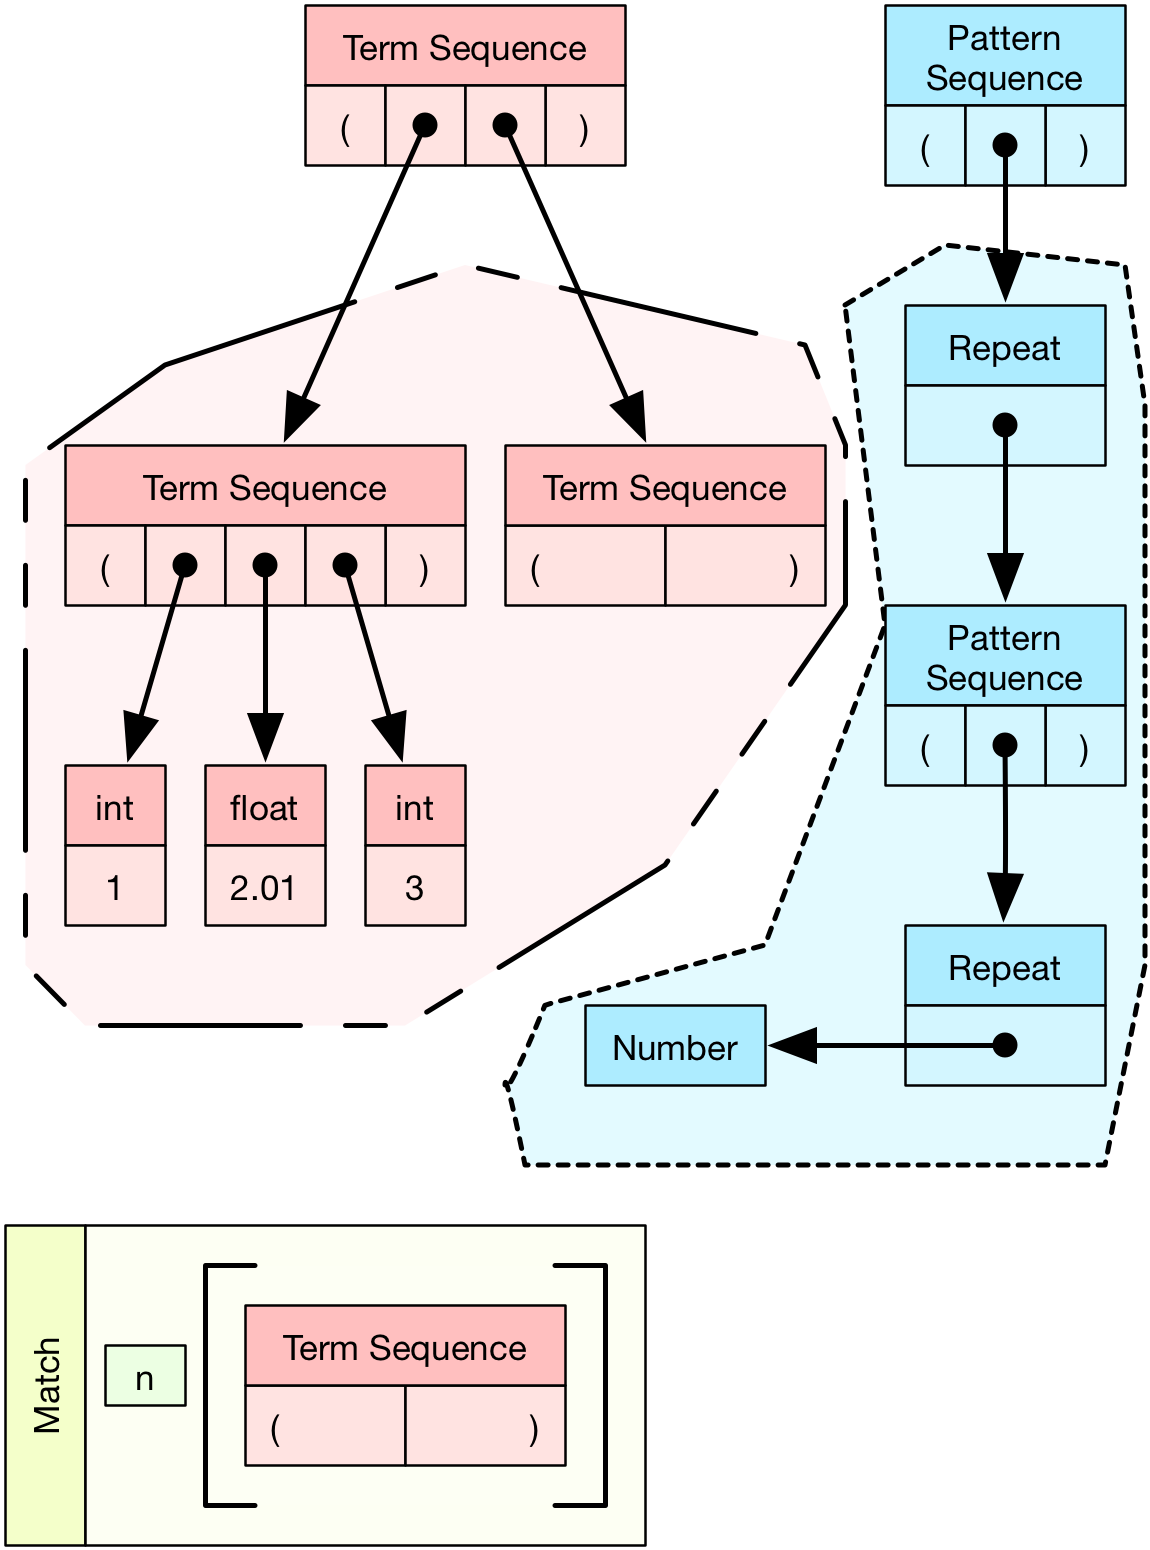
\includegraphics[scale=0.152]{ellipsis-example-fig-b.png}
		\caption{Enter outer ellipsis and \texttt{increasedepth("n")}.}
		\label{ellipsis-example-fig-b}
	\end{subfigure}
}

\fbox{
	\begin{subfigure}{0.5\linewidth}
		\raisebox{19mm}{
			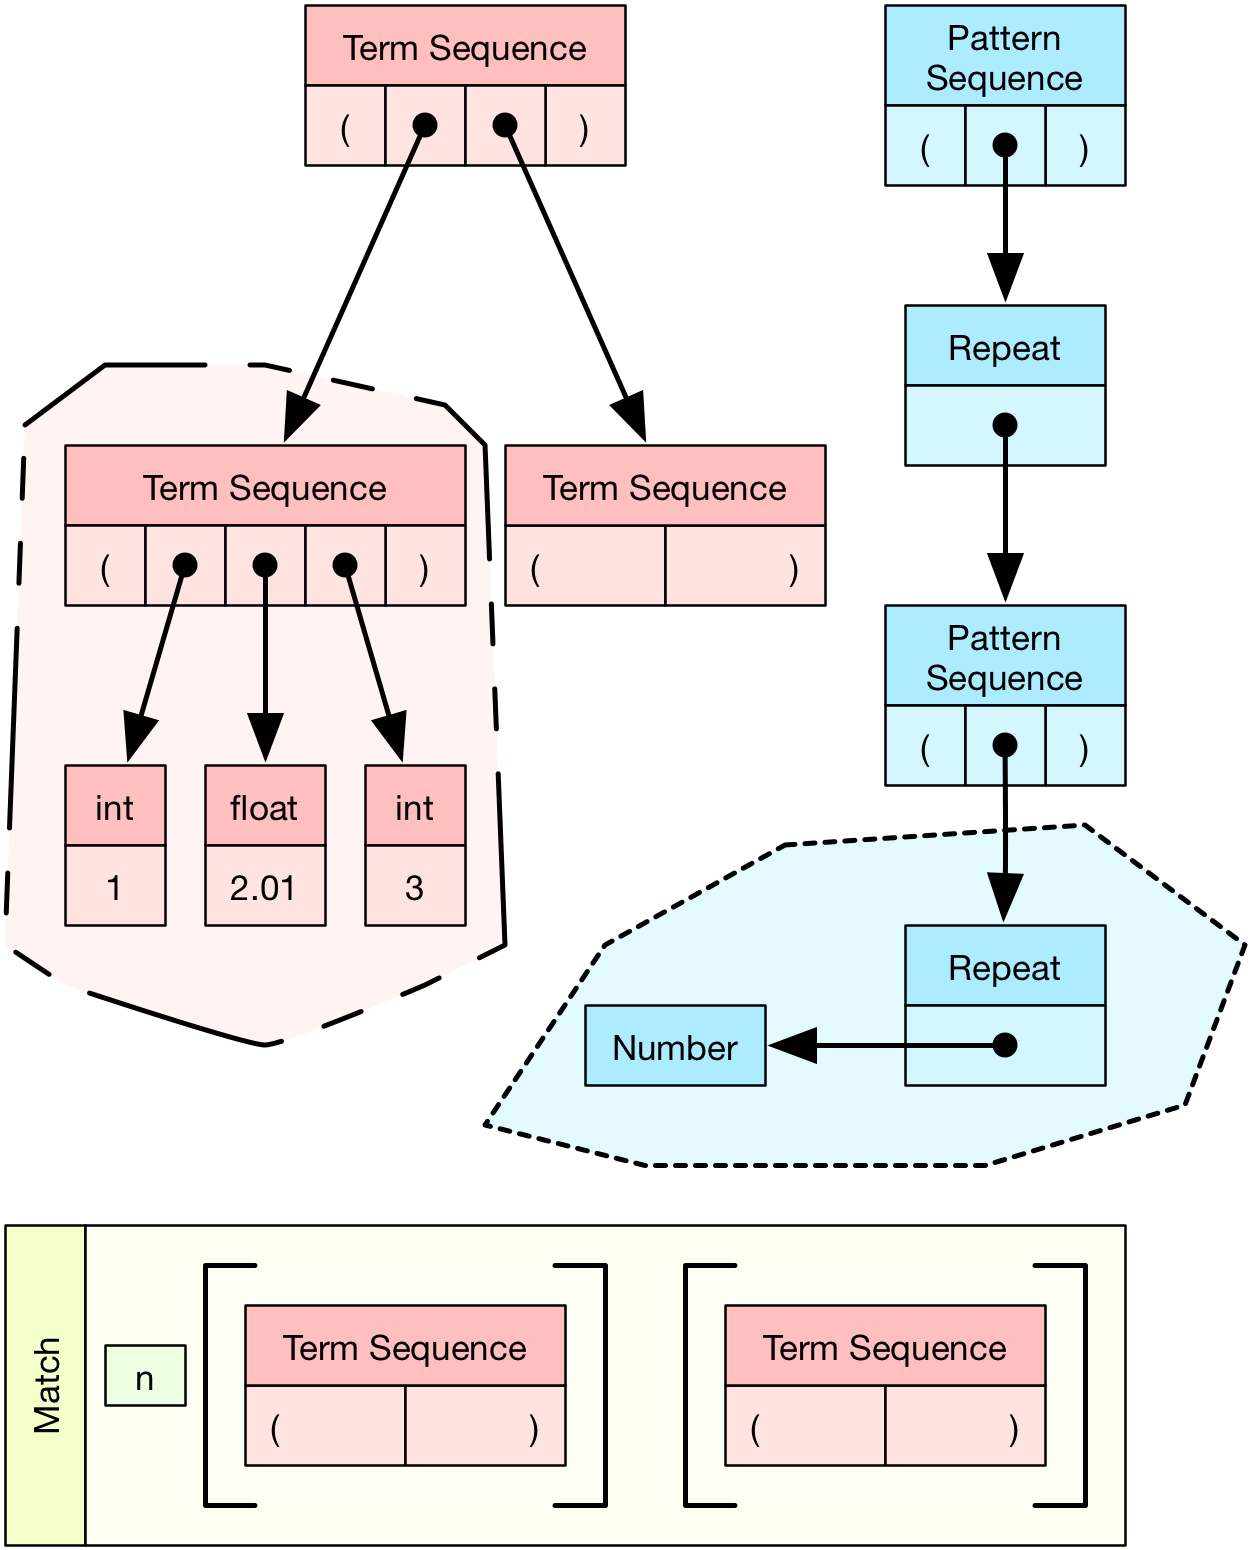
\includegraphics[scale=0.152]{ellipsis-example-fig-c.png}
		}
		\caption{Enter inner ellipsis and \texttt{increasedepth("n")}.}
		\label{ellipsis-example-fig-c}
	\end{subfigure}
	\begin{subfigure}{0.5\linewidth}
		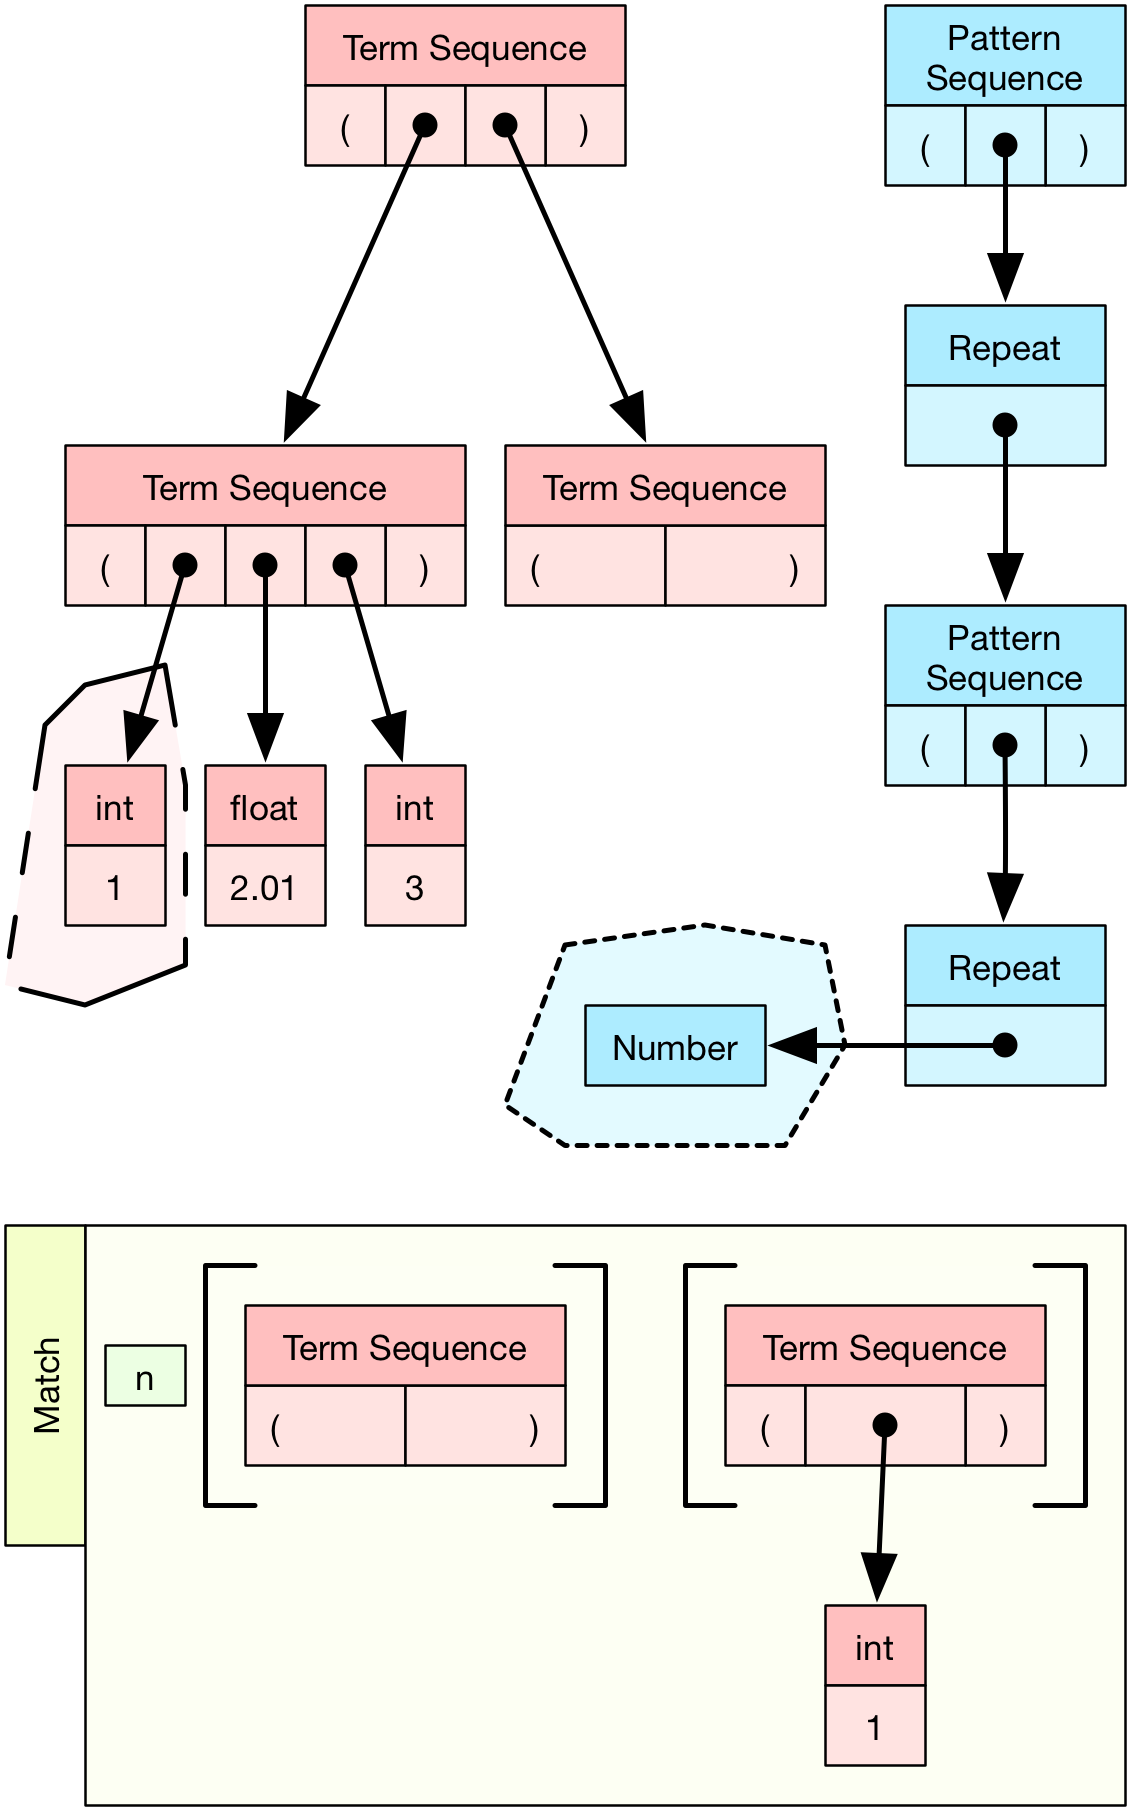
\includegraphics[scale=0.152]{ellipsis-example-fig-d.png}
		\caption{\texttt{addtobinding("n", Integer(1))}}
		\label{ellipsis-example-fig-d}
	\end{subfigure}
}

%\end{adjustwidth}
\end{figure}

\begin{figure}[H]\ContinuedFloat
\fbox{
	\begin{subfigure}{0.5\linewidth}
		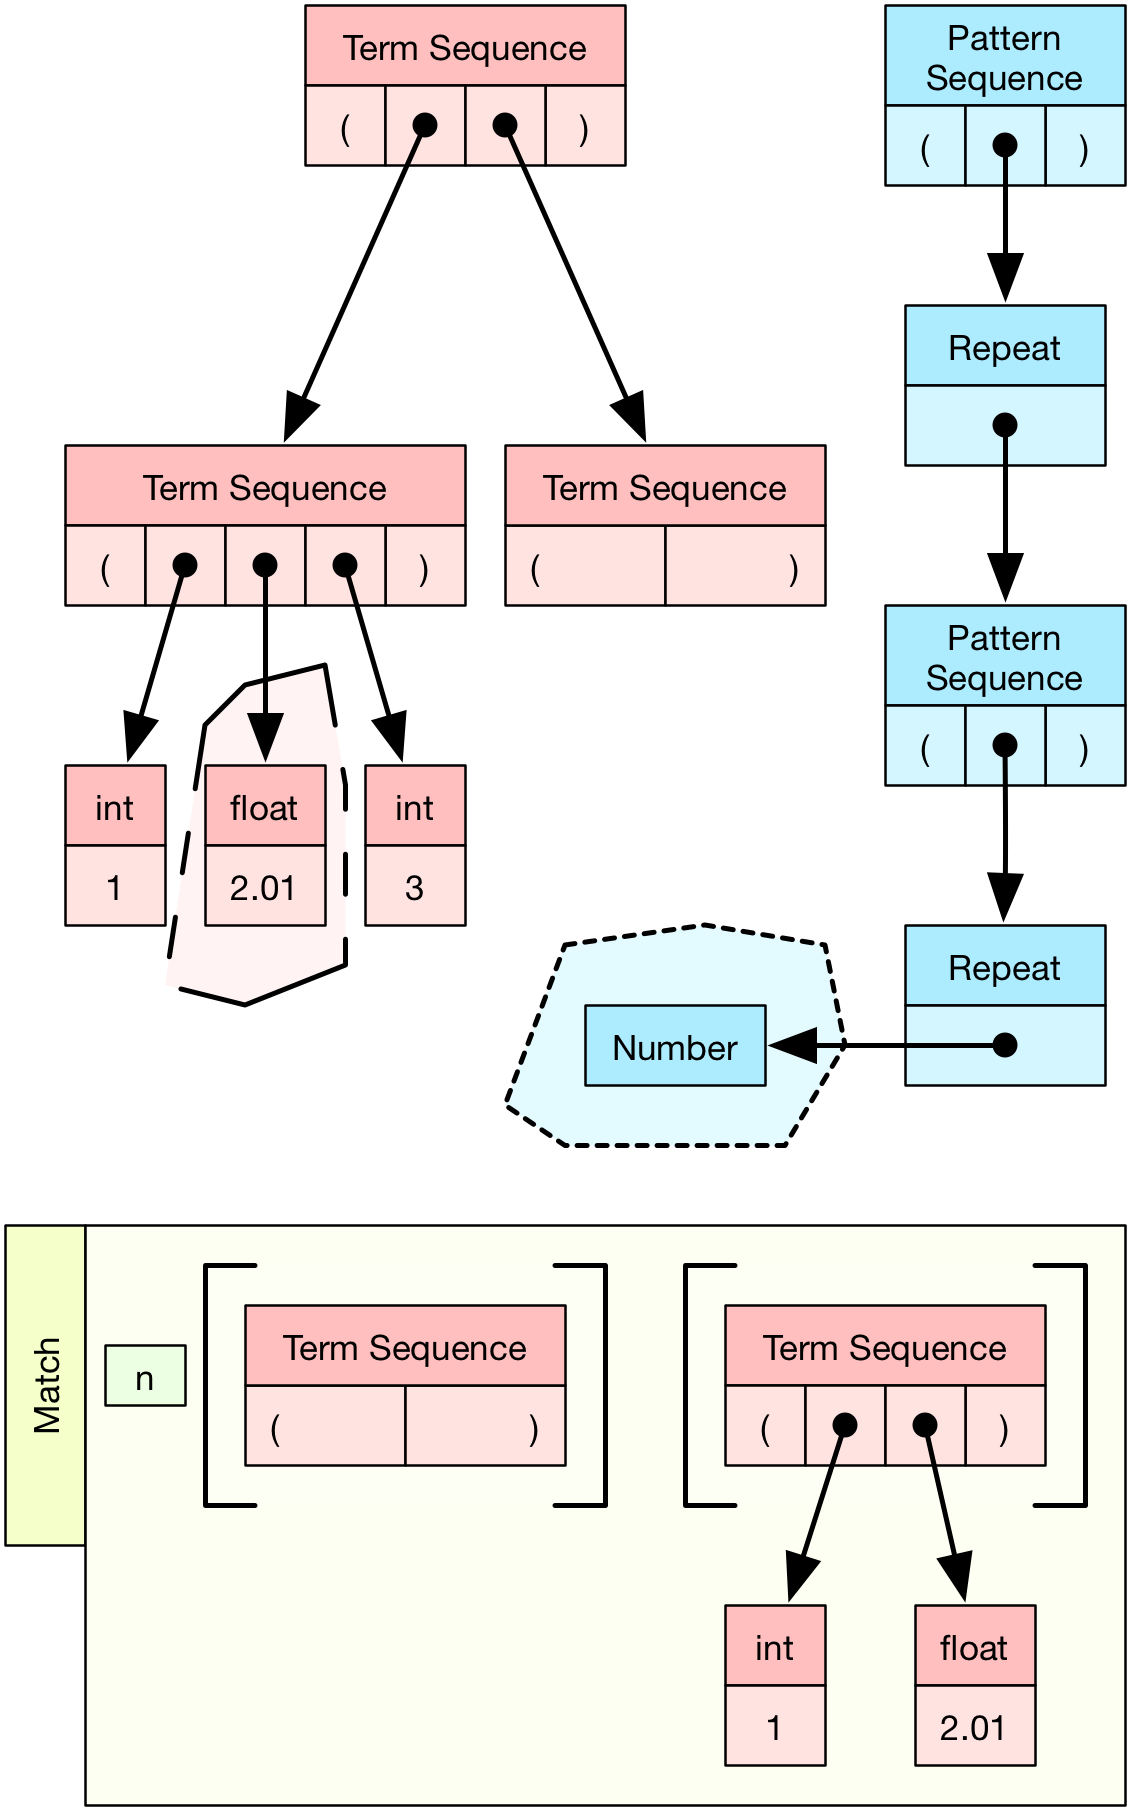
\includegraphics[scale=0.152]{ellipsis-example-fig-e.png}
		\caption{\texttt{addtobinding("n", Float(2.01))}}
		\label{ellipsis-example-fig-e}
	\end{subfigure}
	\begin{subfigure}{0.5\linewidth}
		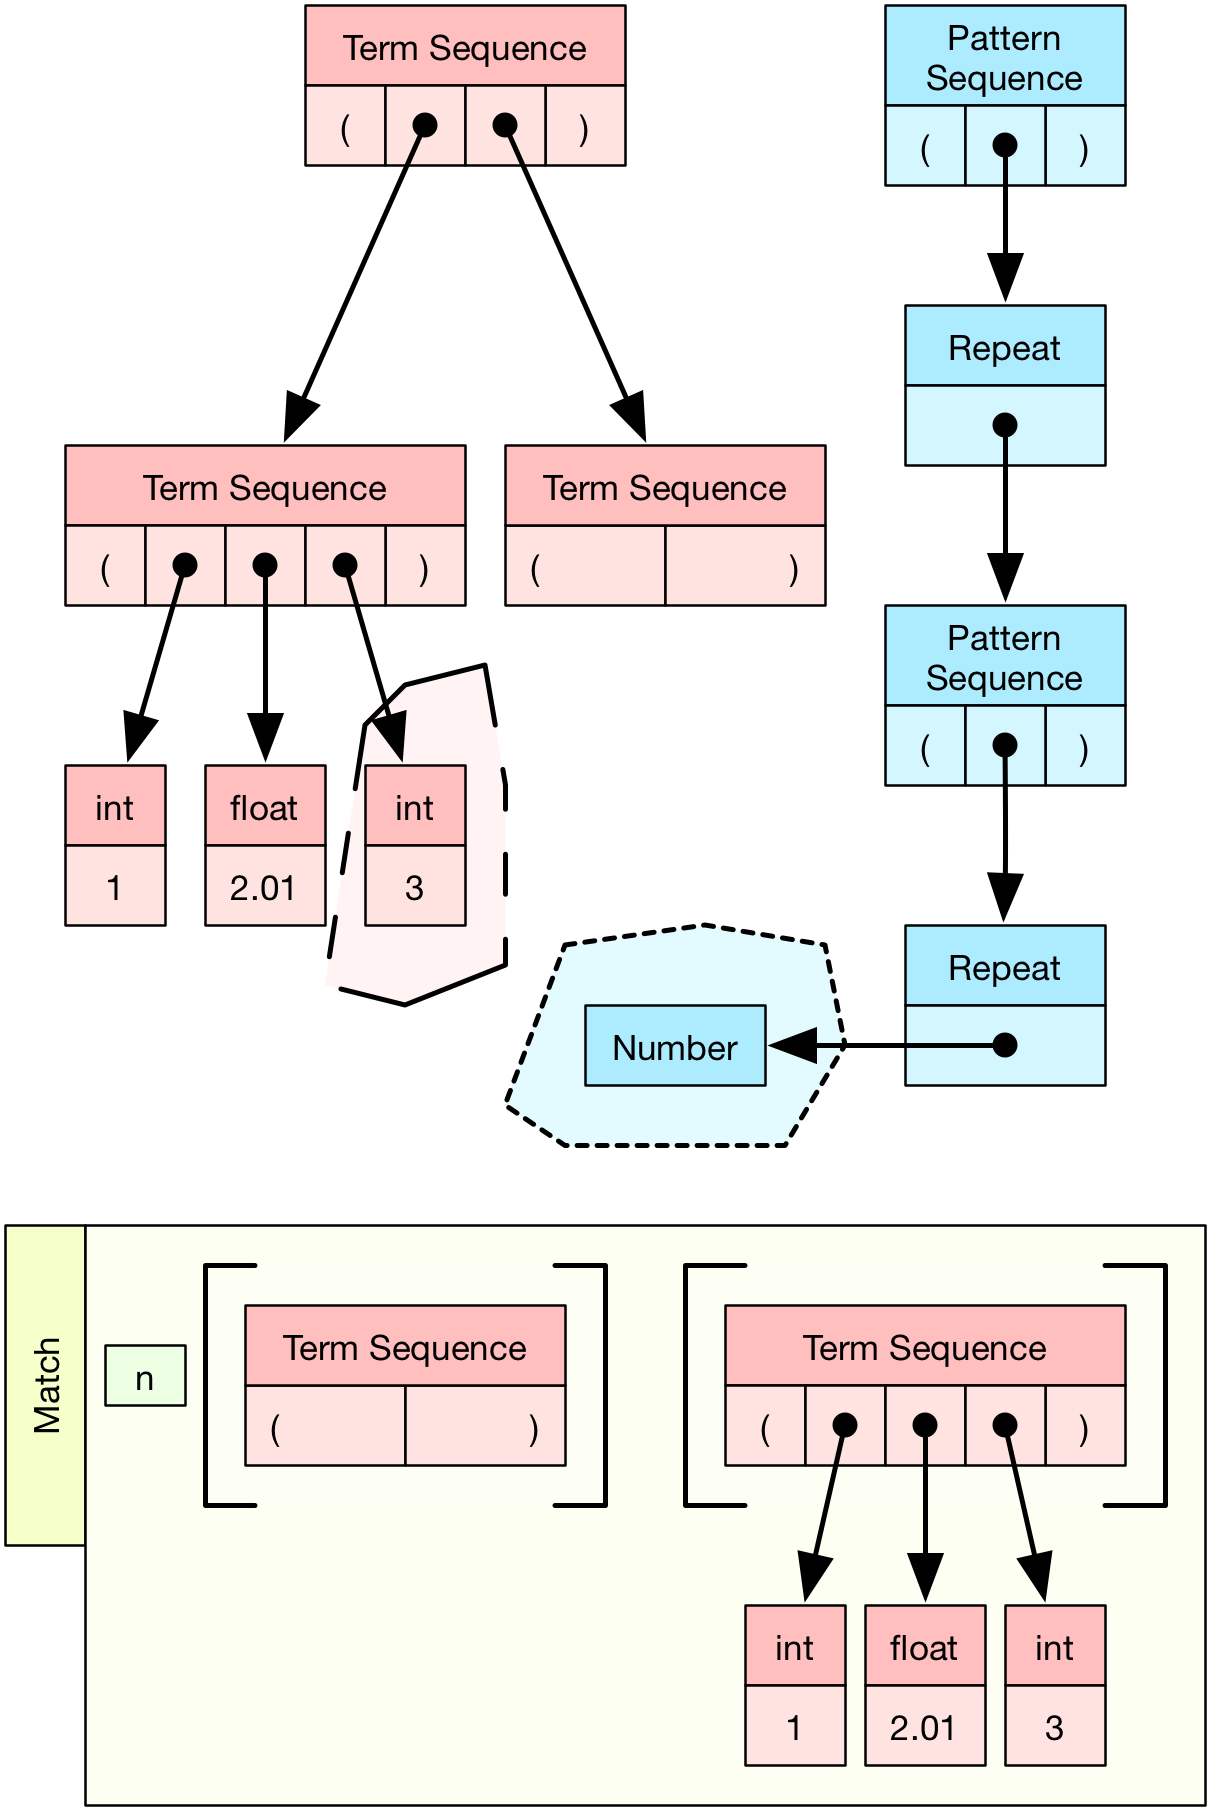
\includegraphics[scale=0.152]{ellipsis-example-fig-f.png}
		\caption{\texttt{addtobinding("n", Integer(3))}}
		\label{ellipsis-example-fig-f}
	\end{subfigure}
}
\fbox{
\begin{subfigure}{0.5\linewidth}
	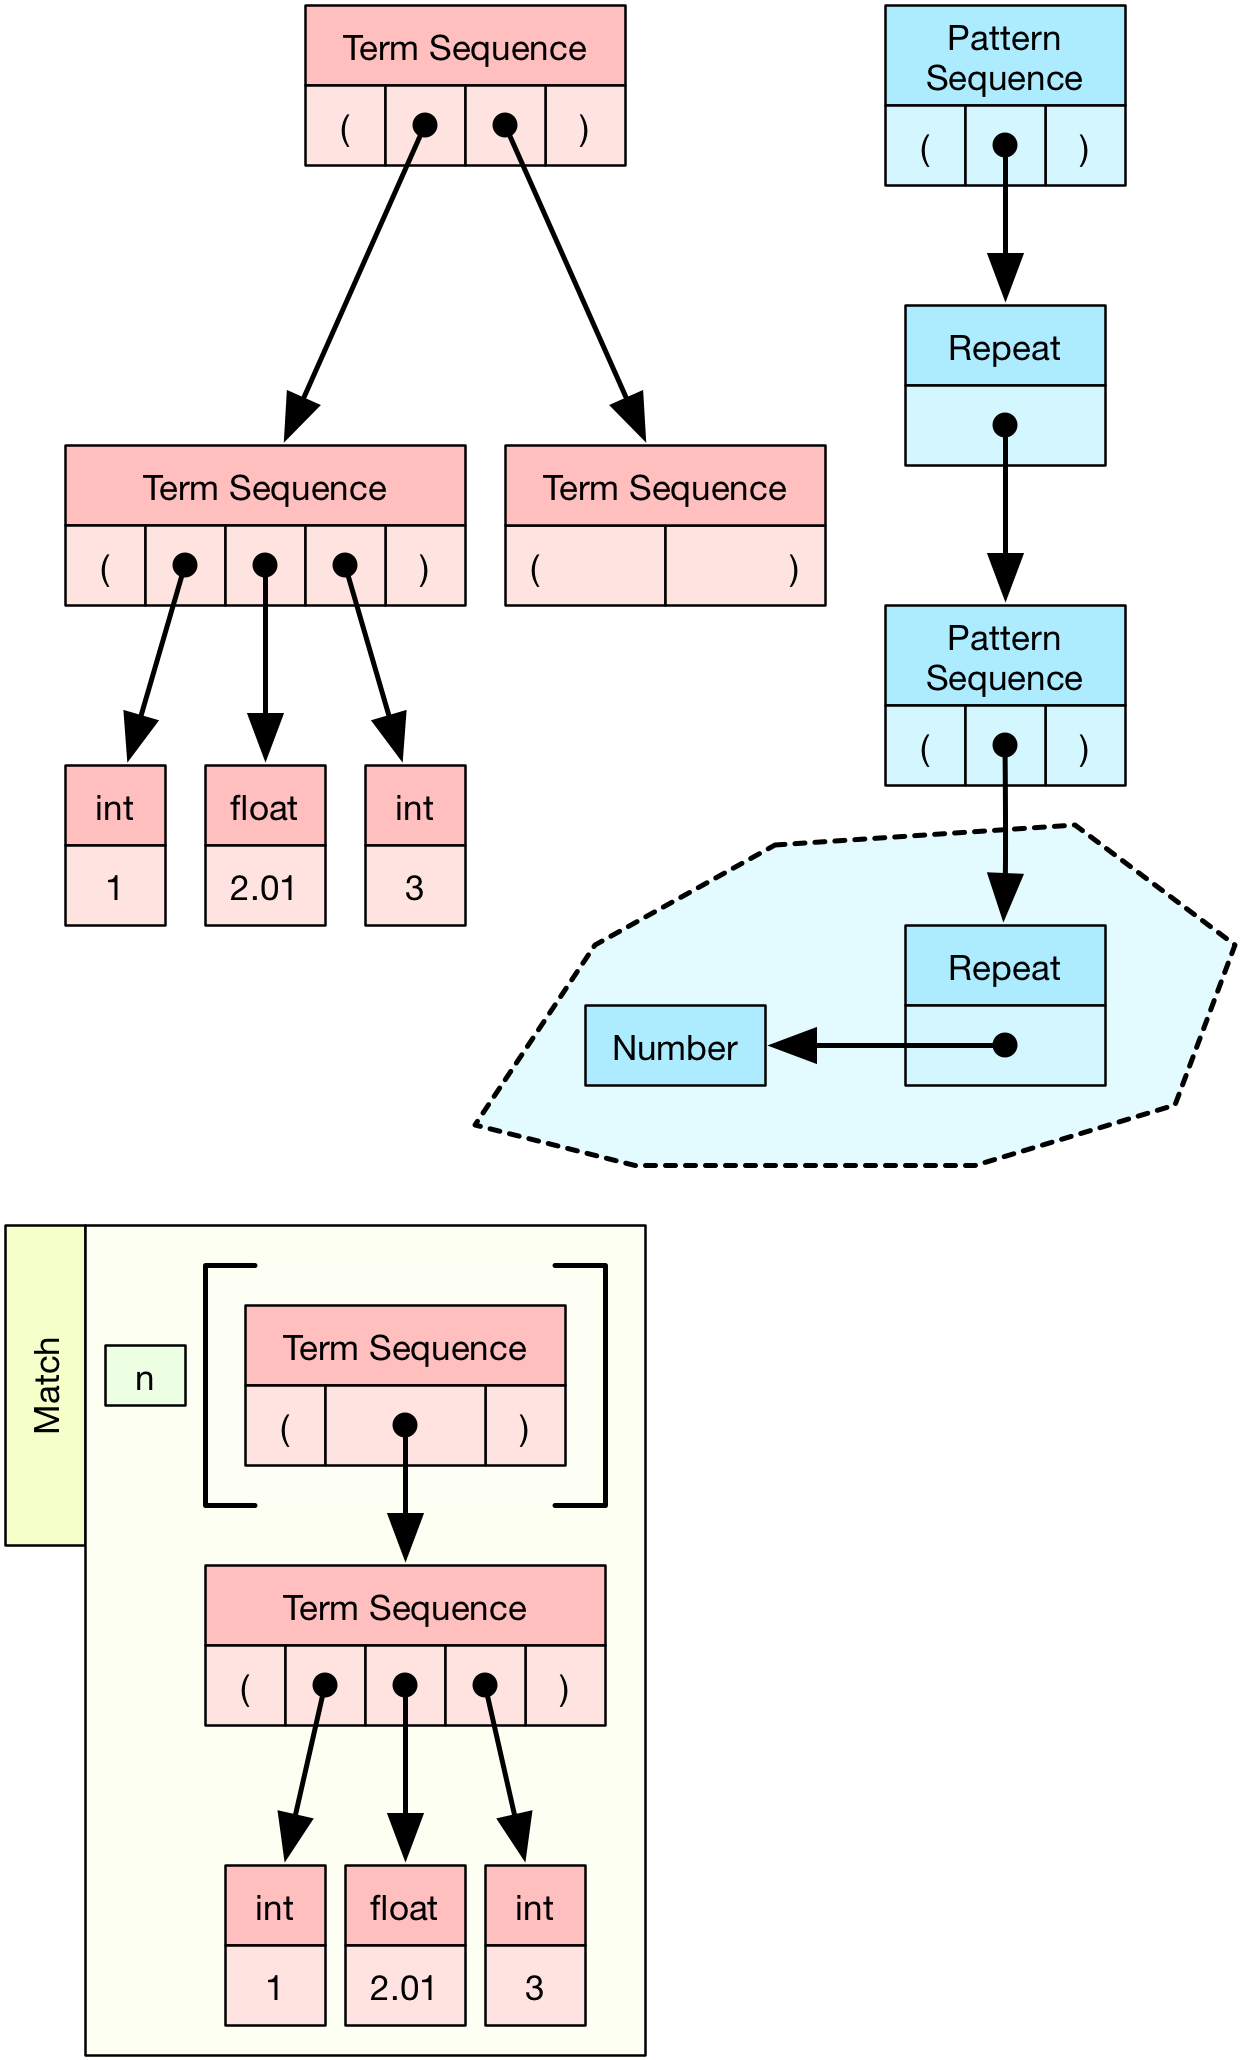
\includegraphics[scale=0.152]{ellipsis-example-fig-g.png}
	\caption{\texttt{decreasedepth("n")} and leave inner ellipsis.}
	\label{ellipsis-example-fig-g}
\end{subfigure}
\begin{subfigure}{0.5\linewidth}
	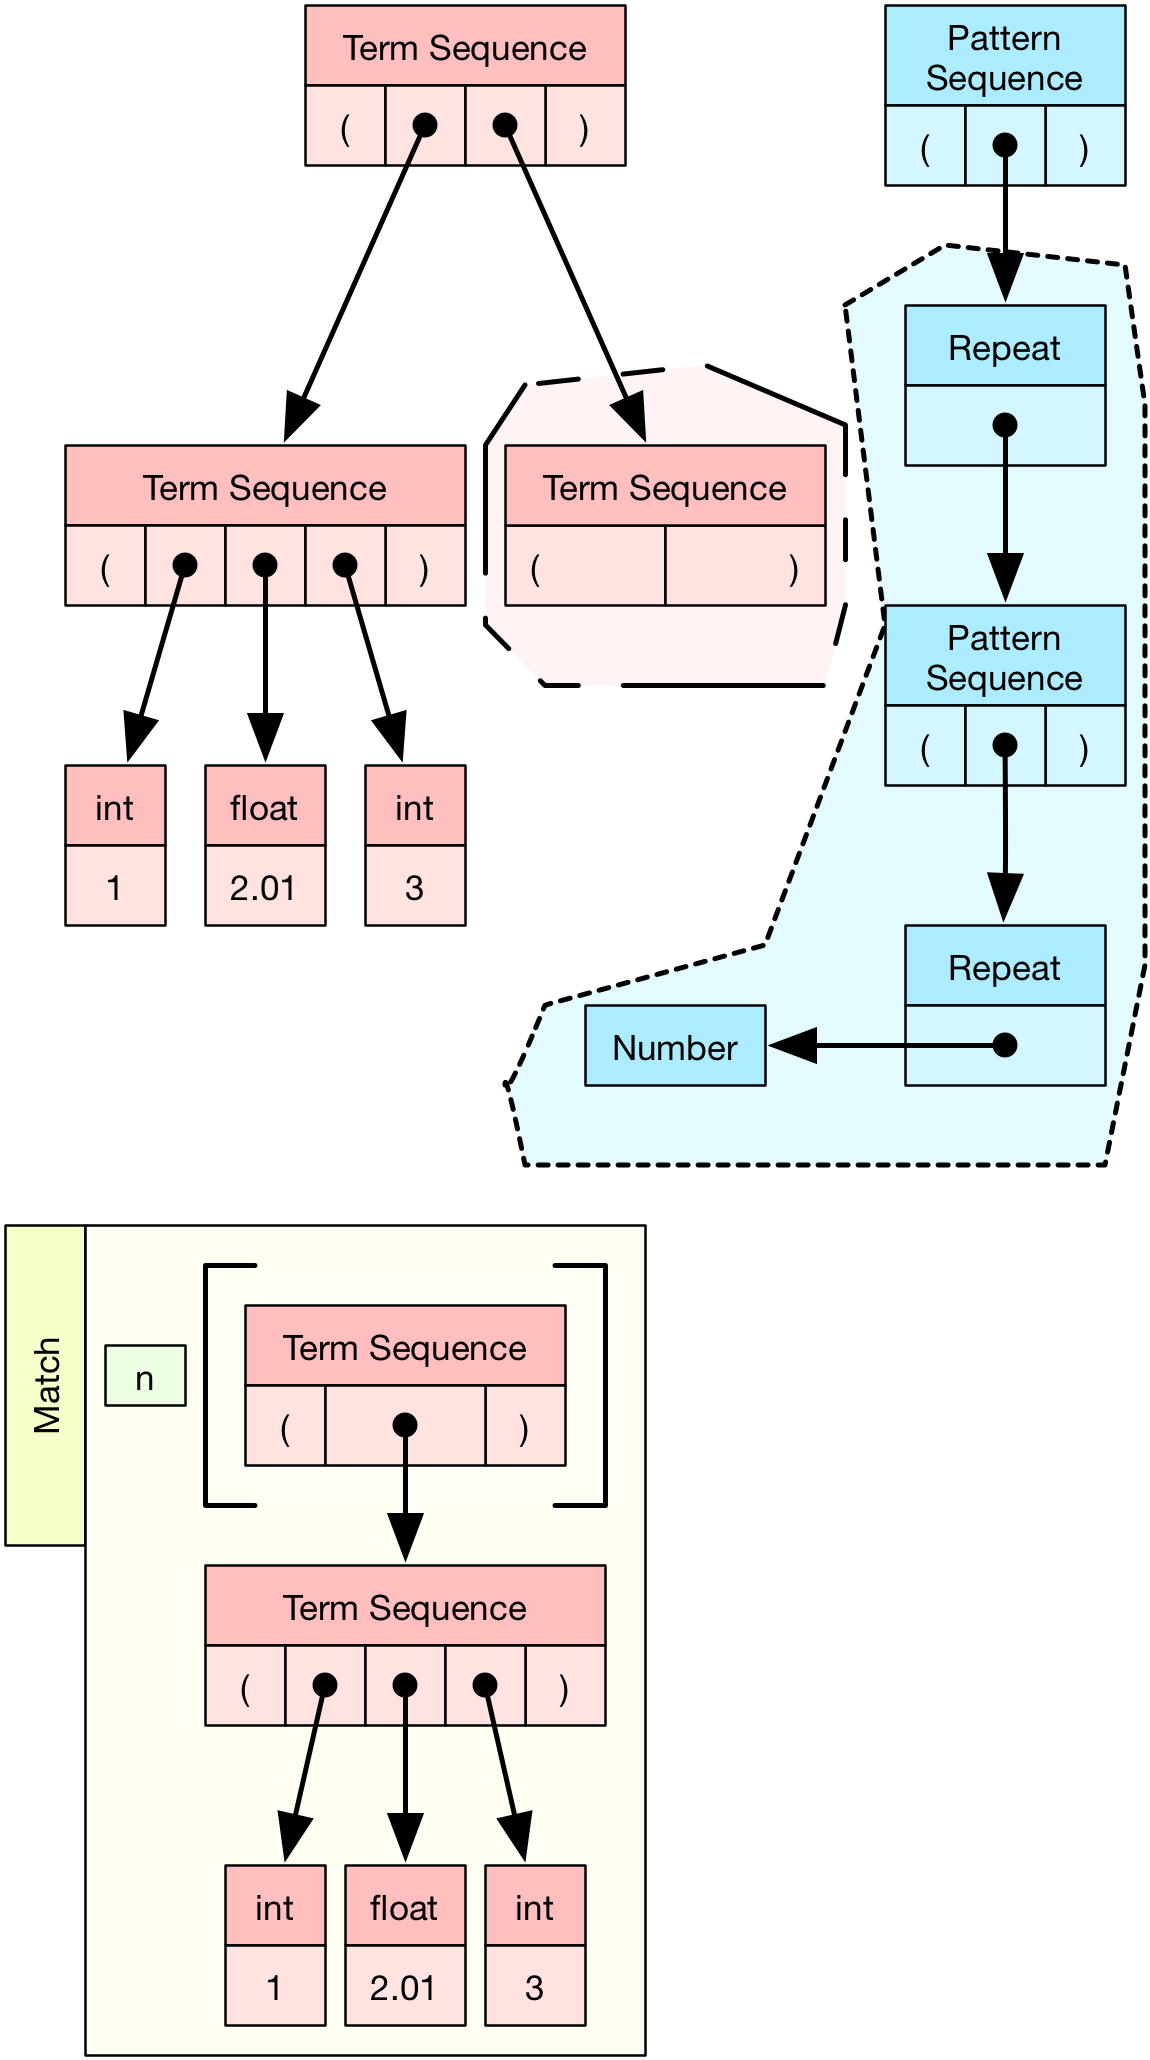
\includegraphics[scale=0.152]{ellipsis-example-fig-h.png}
	\caption{Start processing the next term in the sequence.}
	\label{ellipsis-example-fig-h}
\end{subfigure}
}
\end{figure}
\begin{figure}[H]\ContinuedFloat
\fbox{
	\begin{subfigure}{0.5\linewidth}
		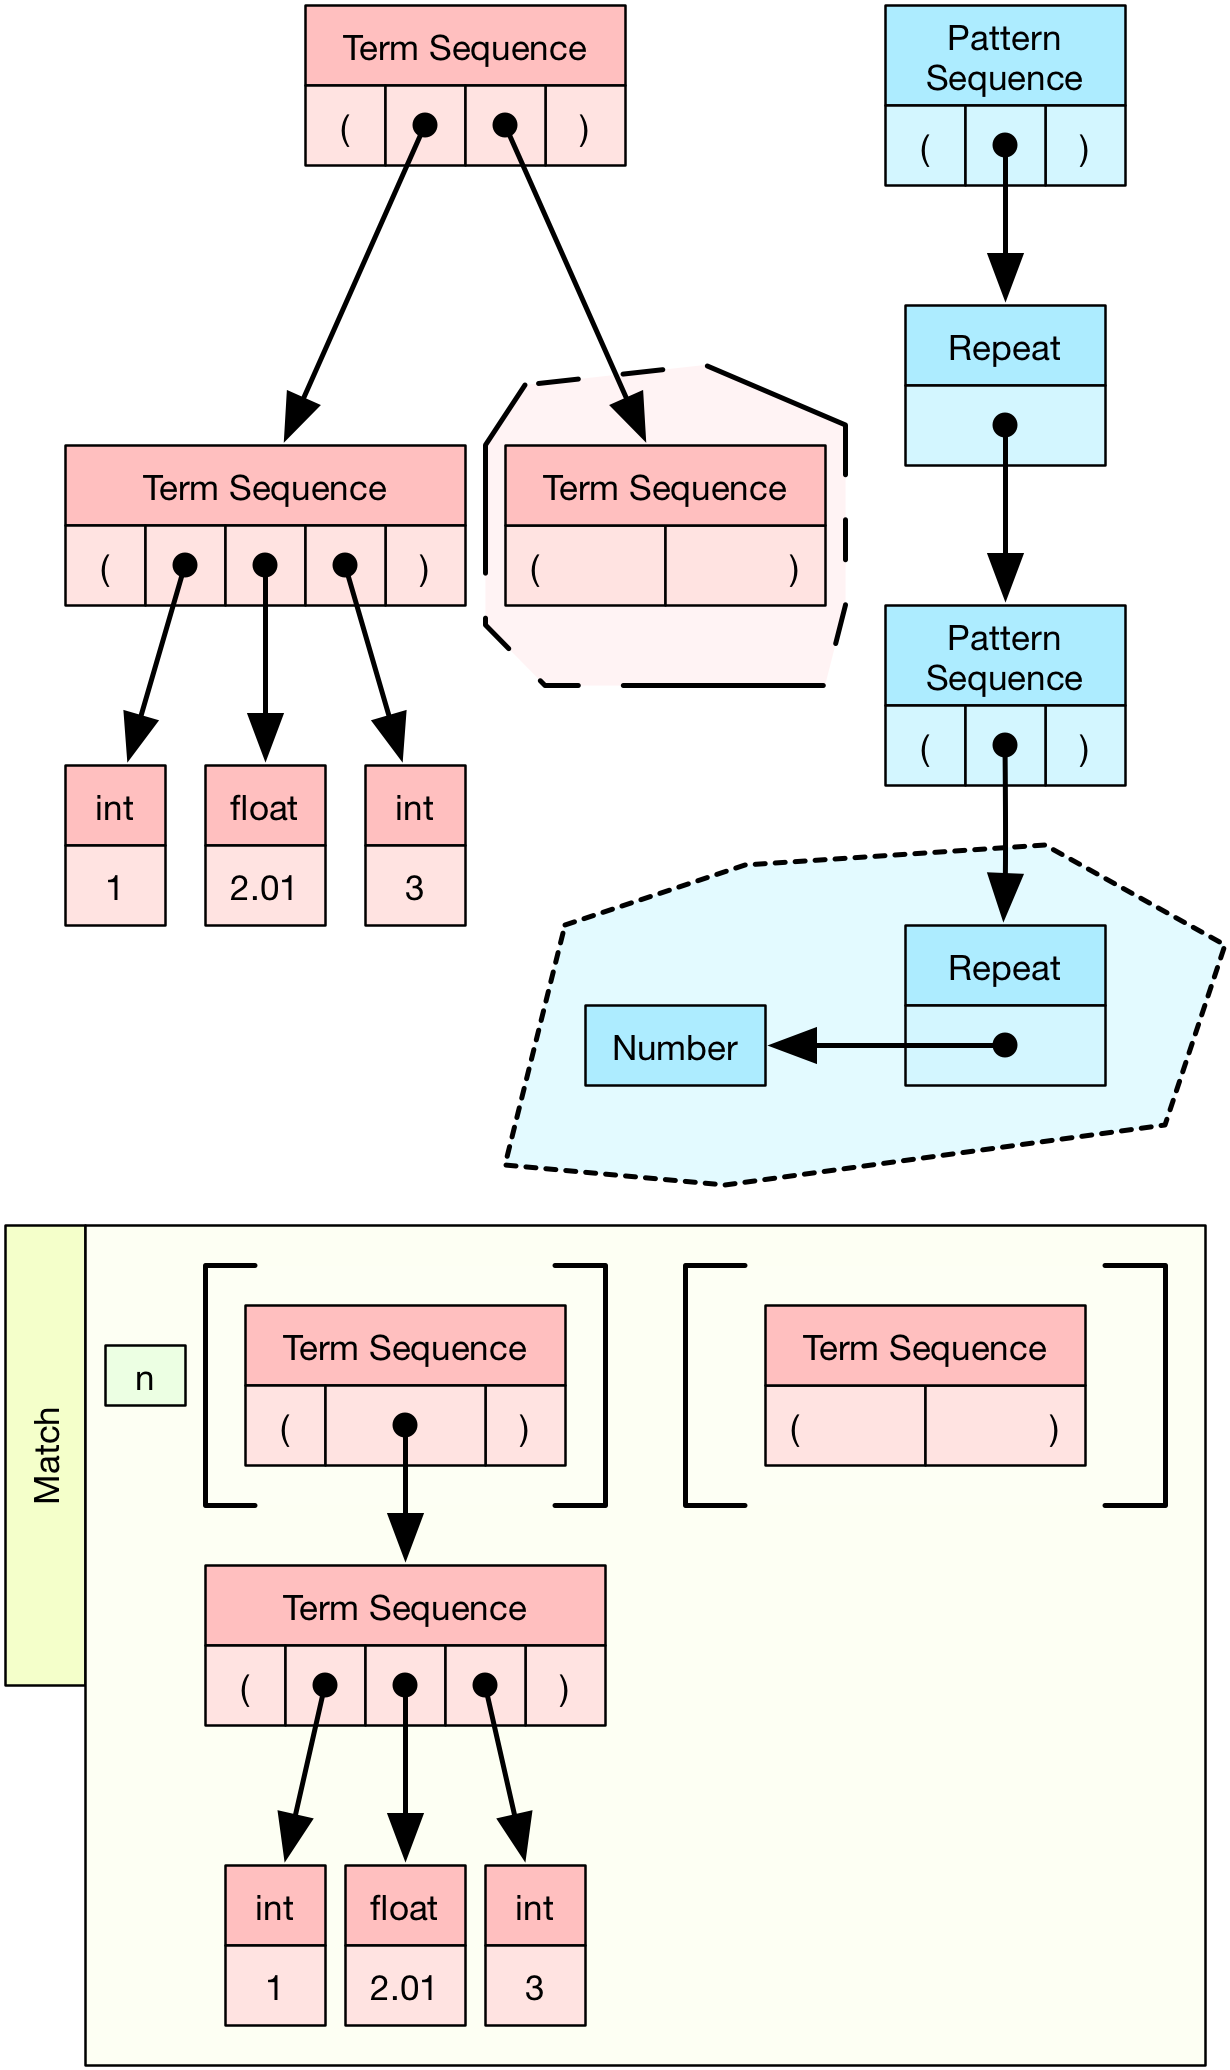
\includegraphics[scale=0.152]{ellipsis-example-fig-i.png}
		\caption{\texttt{increasedepth("n")} after entering inner ellipsis.}
		\label{ellipsis-example-fig-i}
	\end{subfigure}
	\begin{subfigure}{0.5\linewidth}
		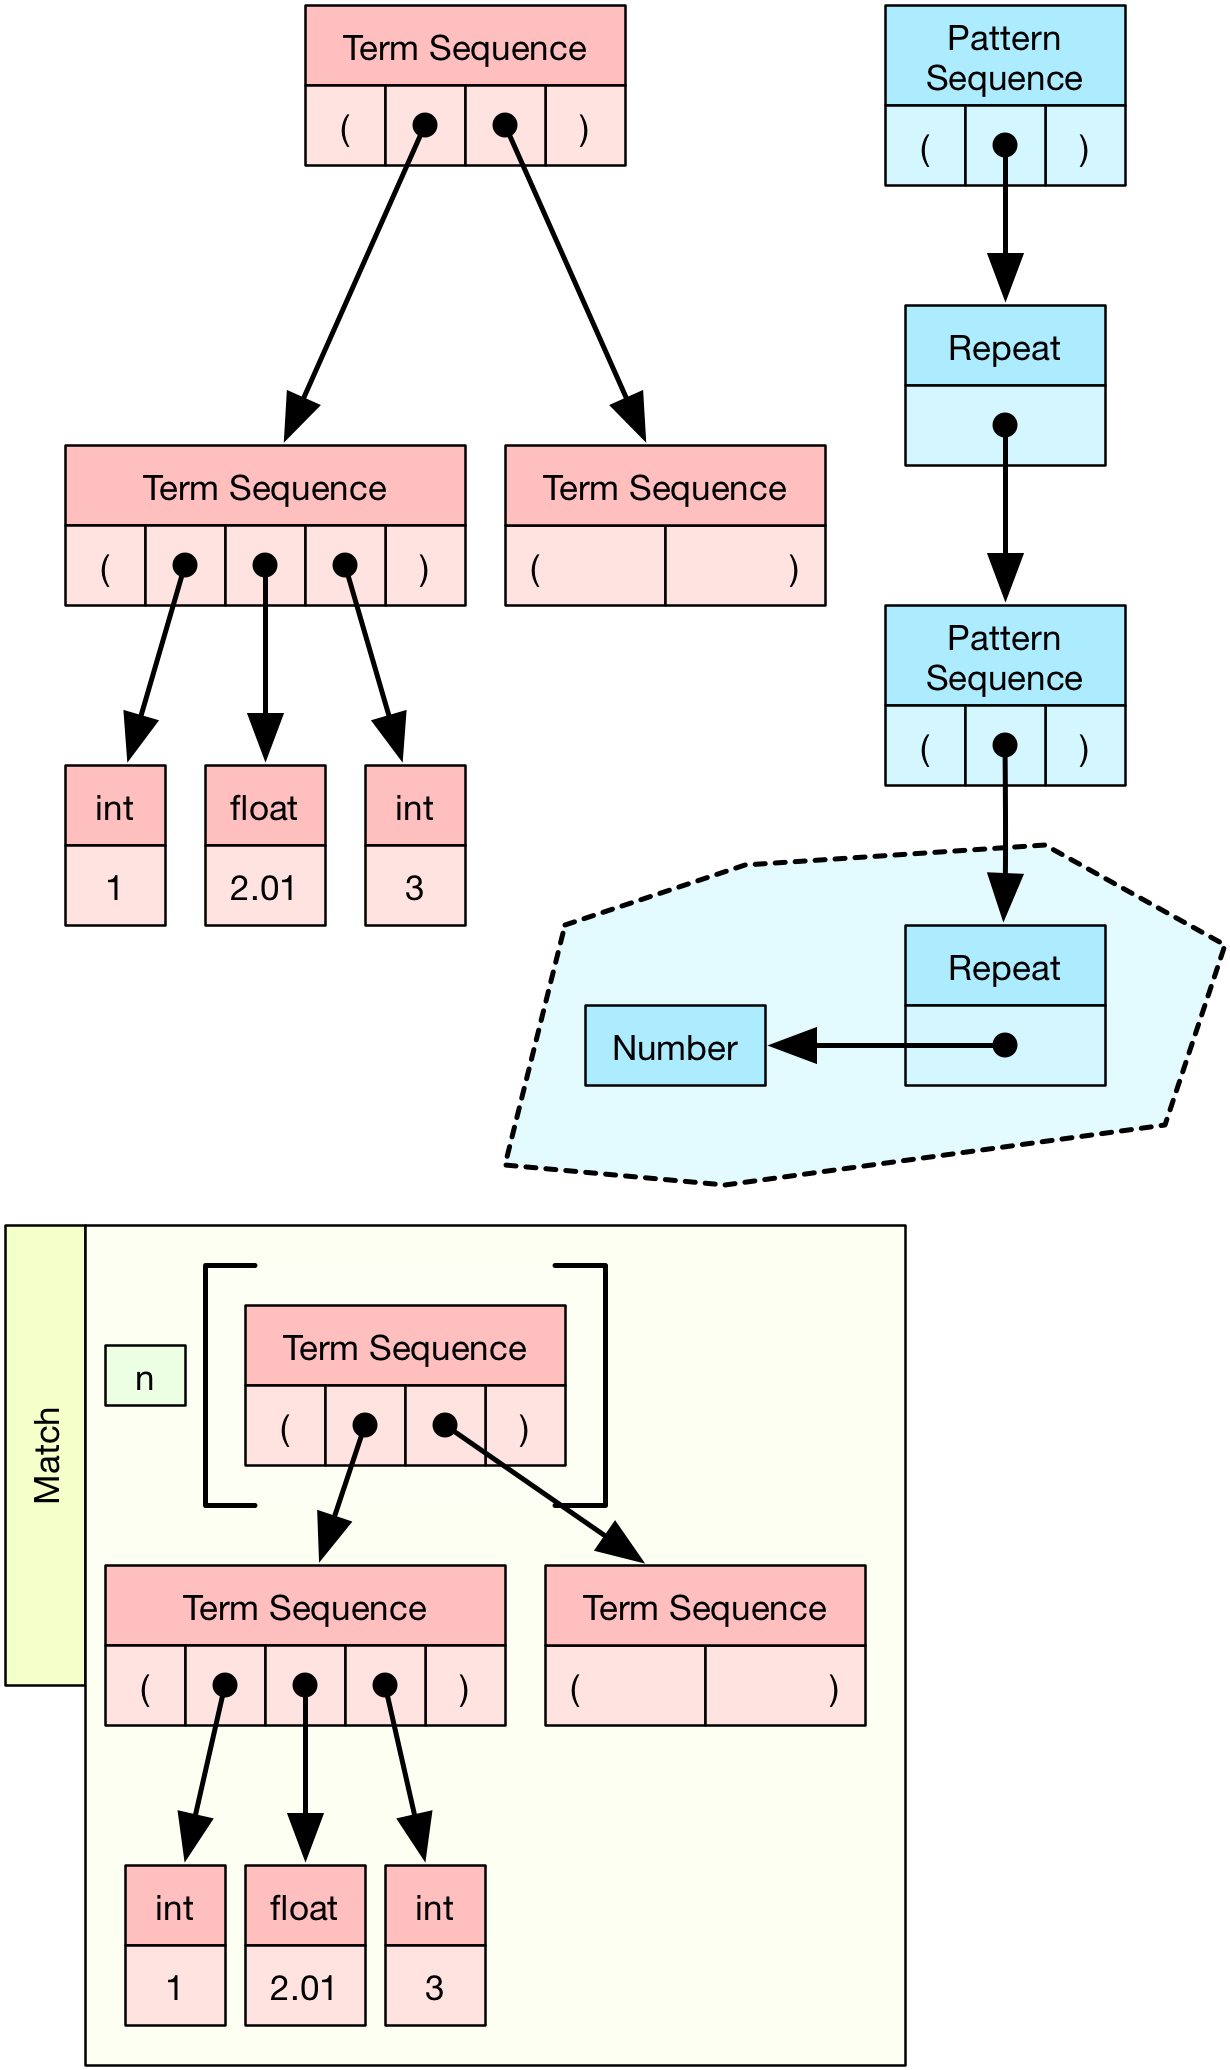
\includegraphics[scale=0.152]{ellipsis-example-fig-j.png}
		\caption{\texttt{decreasedepth("n")} and leave inner ellipsis.}
		\label{ellipsis-example-fig-j}
	\end{subfigure}
}

\fbox{
	\begin{subfigure}{0.5\linewidth}
		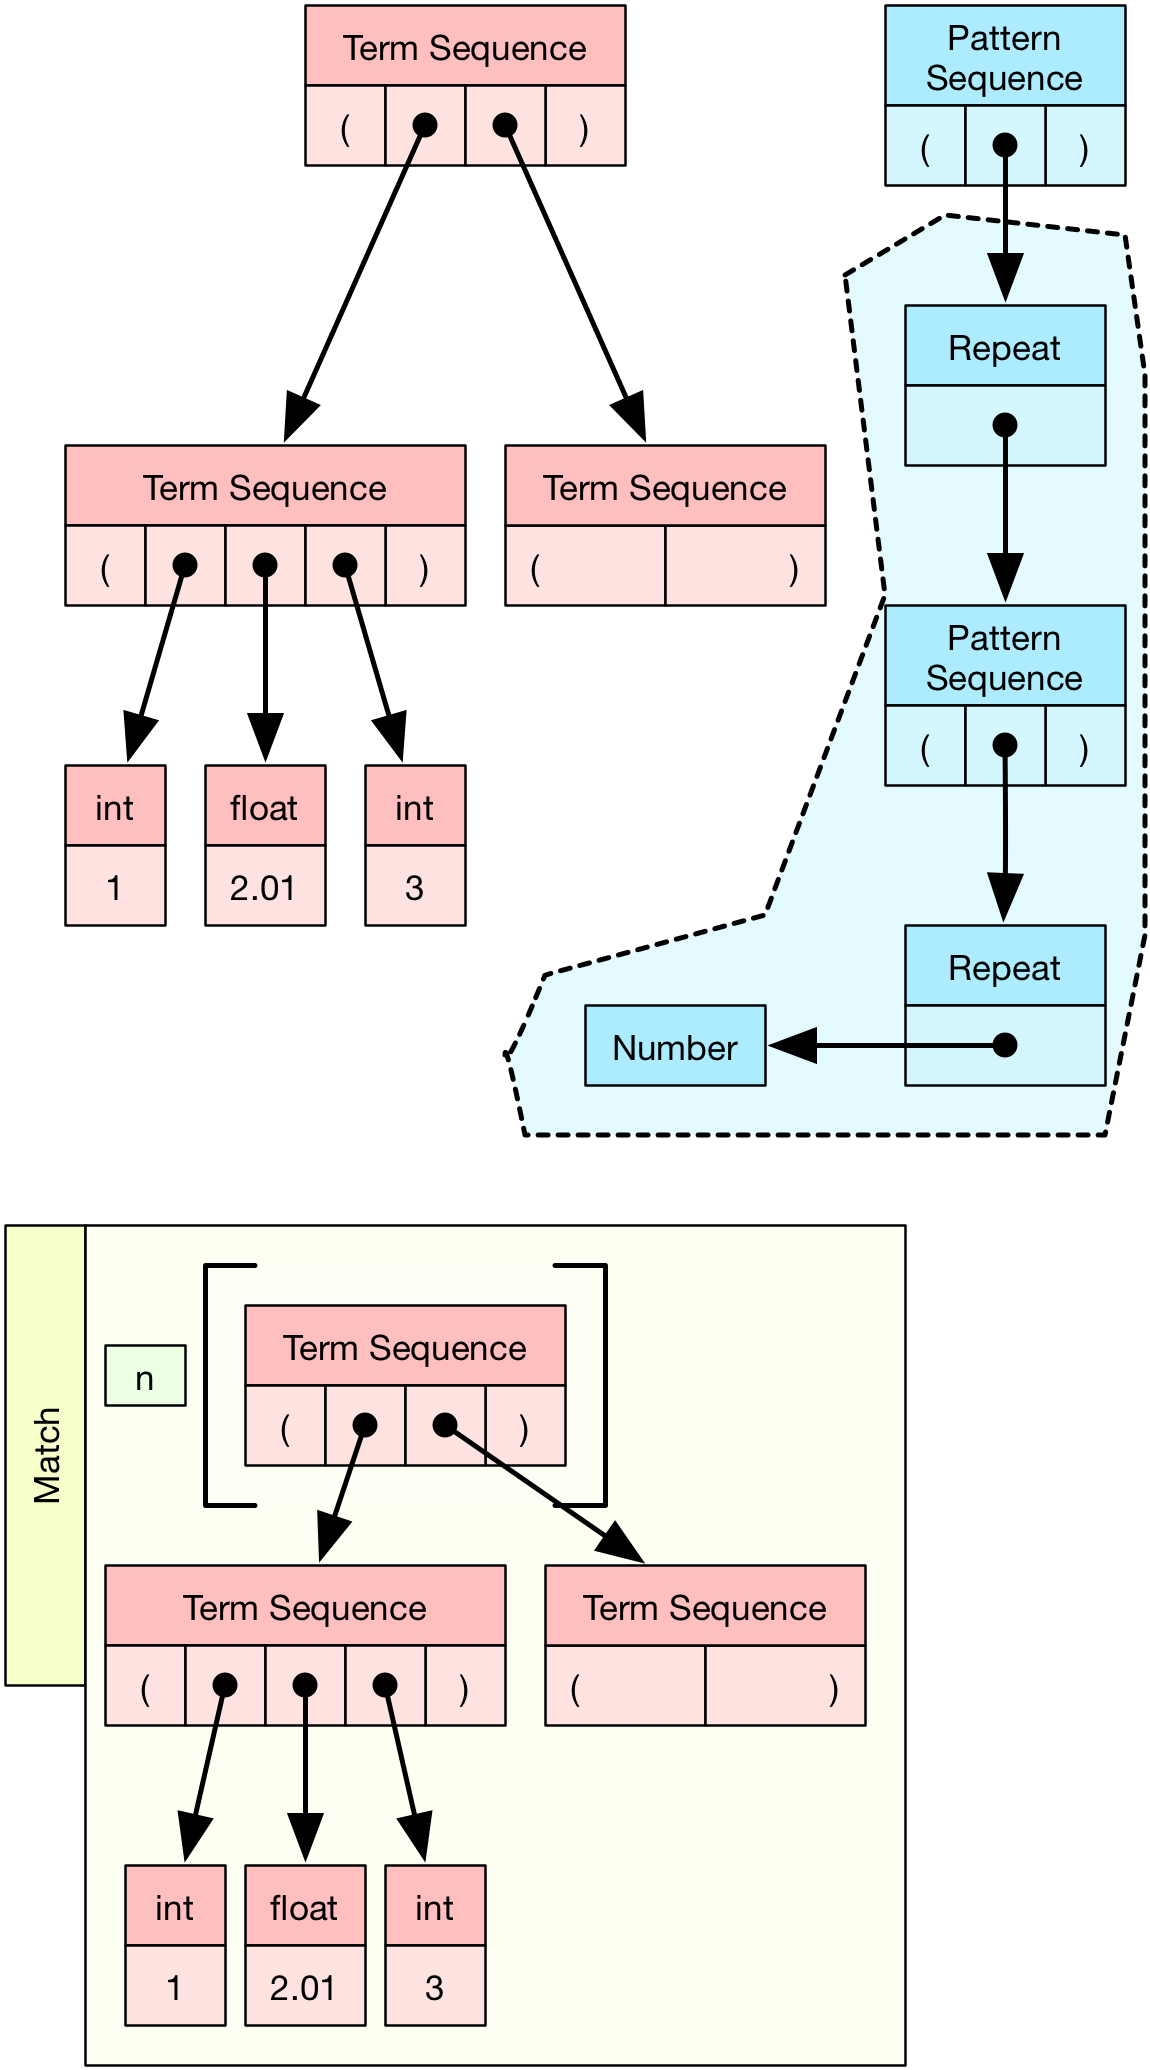
\includegraphics[scale=0.152]{ellipsis-example-fig-k.png}
		\caption{\texttt{decreasedepth("n") and leave outer ellipsis}.}
		\label{ellipsis-example-fig-k}
	\end{subfigure}
}

\end{figure}

\begin{figure}[h]
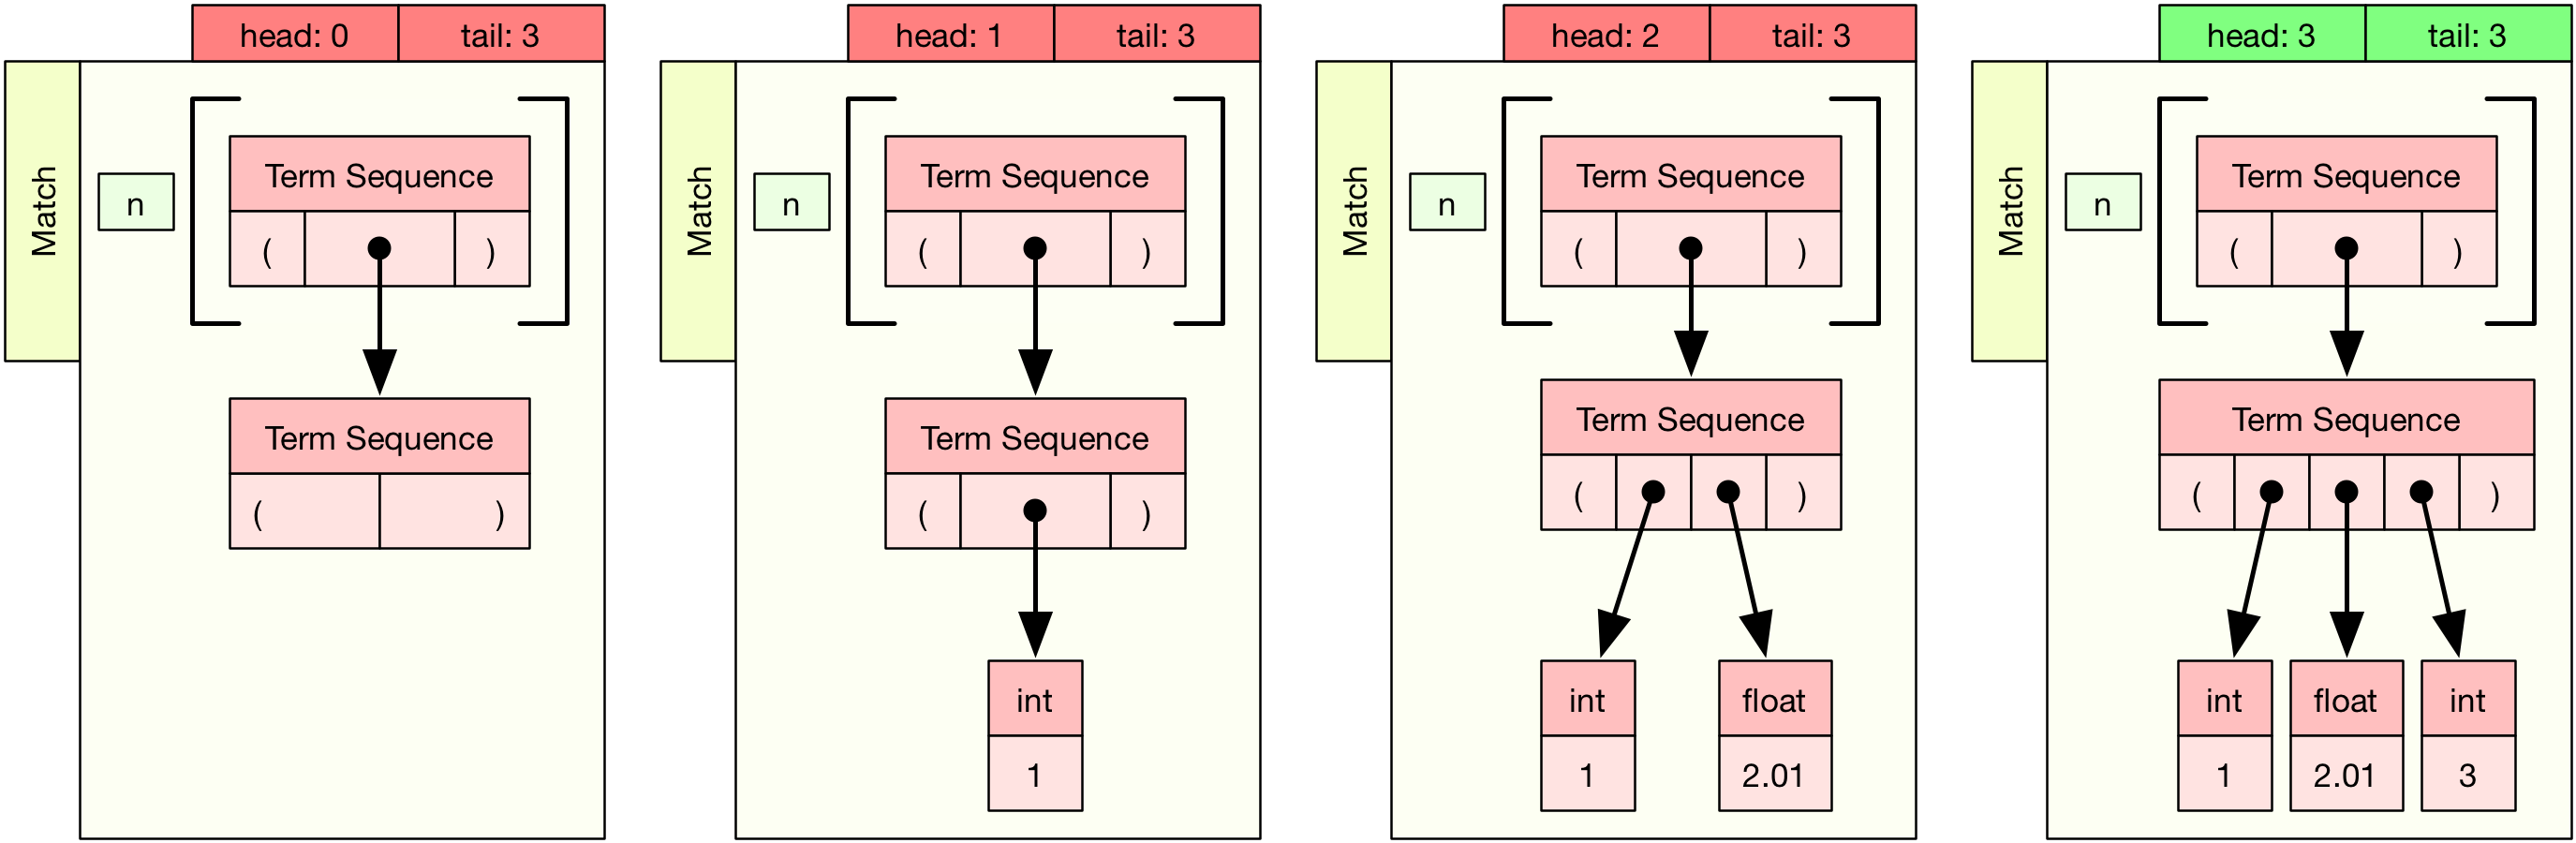
\includegraphics[scale=0.152]{ellipsis-example-matches-1.png}
\caption{Matches returned after matching term \texttt{(1 2 3)} against pattern \texttt{n ...}}
\label{ellipsis-example-matches-1}
\end{figure}


\begin{figure}[h]
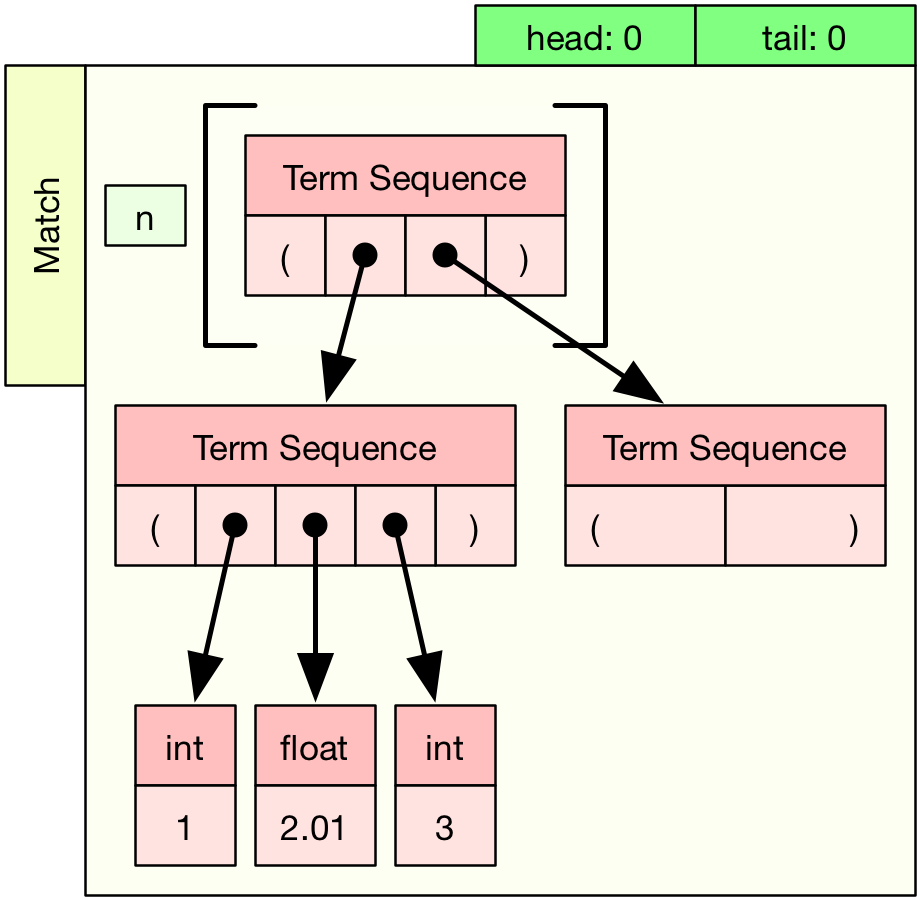
\includegraphics[scale=0.152]{ellipsis-example-matches-2.png}
\caption{Matches returned after matching term \texttt{()} against pattern \texttt{n ...}}
\label{ellipsis-example-matches-2}
\end{figure}

\begin{figure}[h]
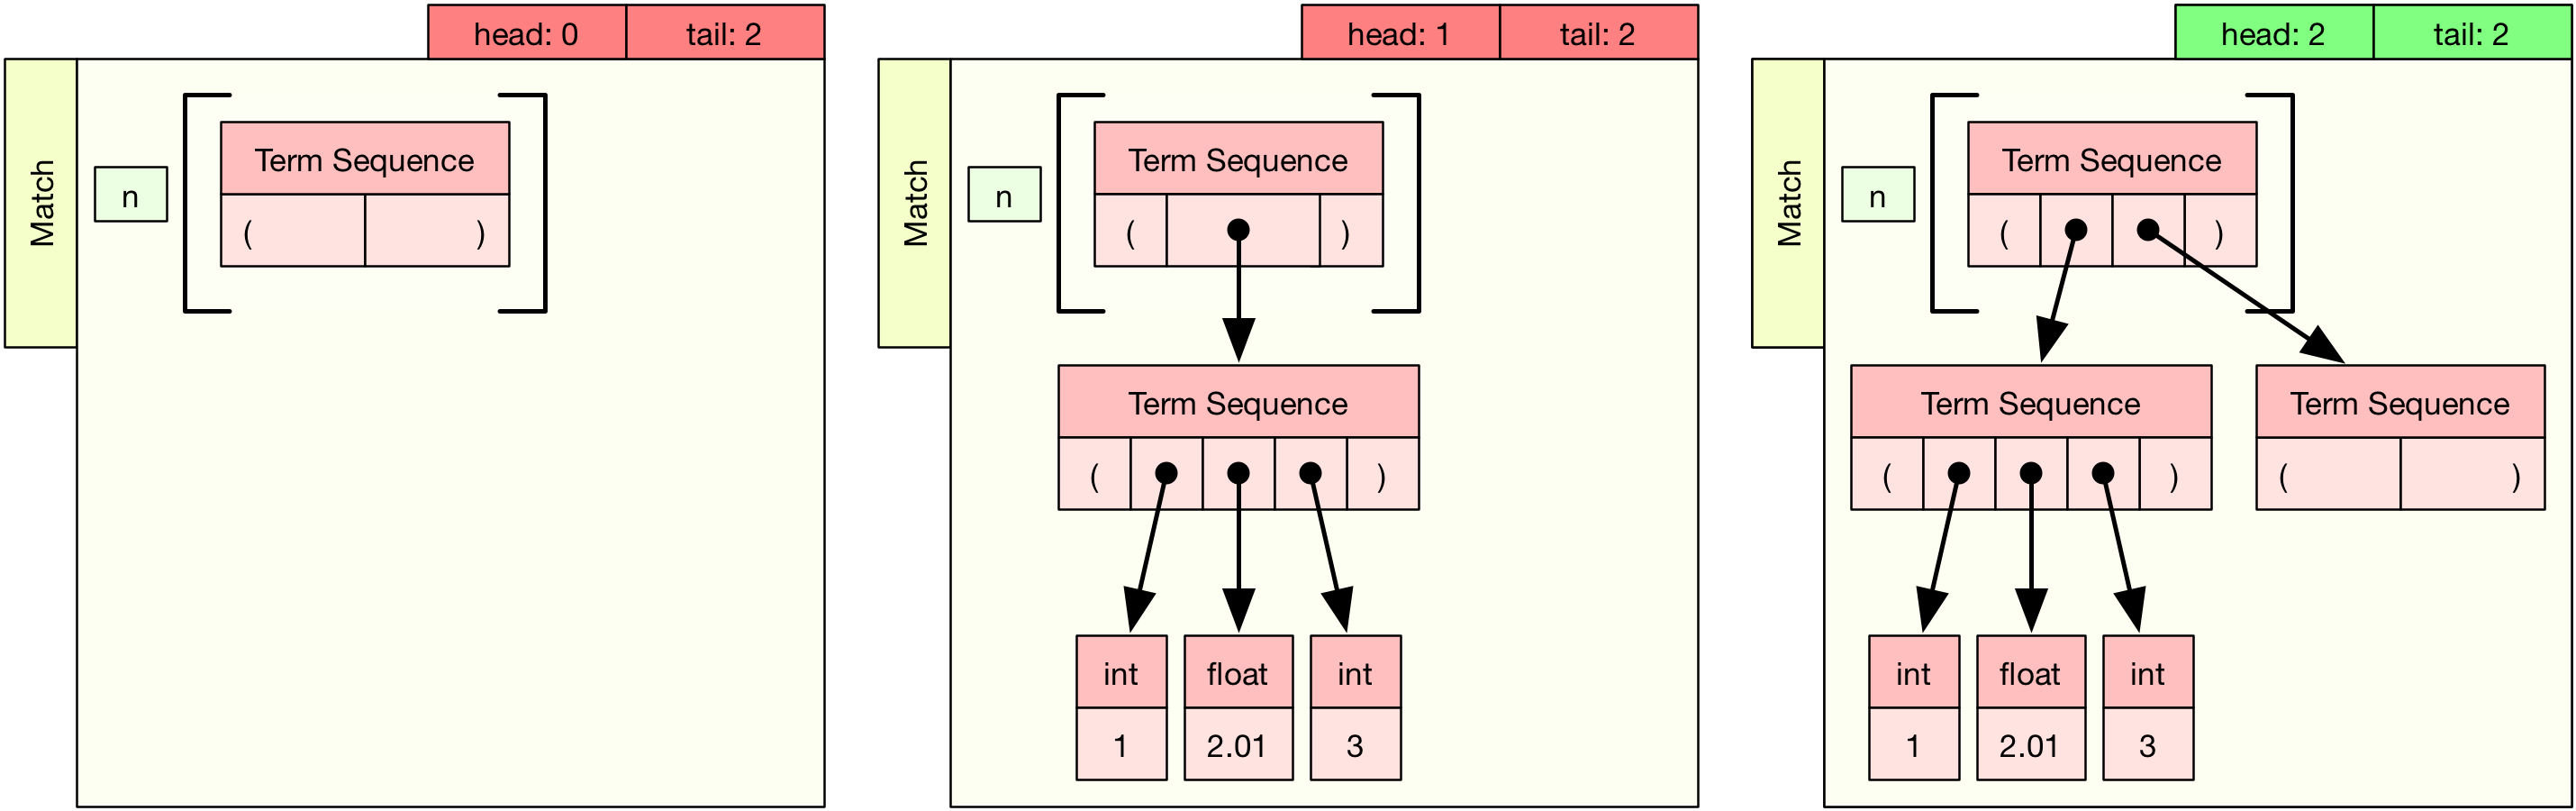
\includegraphics[scale=0.152]{ellipsis-example-matches-3.png}
\caption{Matches returned after matching term \texttt{((1 2 3)())} against pattern \texttt{(n ...) ...} }
\label{ellipsis-example-matches-3}
\end{figure}


